\documentclass[11pt,a4paper]{article}

% Packages
\usepackage[utf8]{inputenc}
\usepackage[spanish, es-tabla]{babel}
\usepackage{caption}
\usepackage{listings}
\usepackage{adjustbox}
\usepackage{enumitem}
\usepackage{hyperref}
\usepackage{boldline}
\usepackage{amsmath}
\usepackage{amssymb, amsmath}
\usepackage[margin=1in]{geometry}
\usepackage{xlop}
\usepackage{soul}
\usepackage[ruled,vlined,linesnumbered]{algorithm2e}
\usepackage{amsthm} %Paquete para la terminología matemática
\usepackage[ruled,vlined,linesnumbered]{algorithm2e}
\usepackage{subfigure}
\usepackage{listings}
\usepackage{color}
\usepackage{float}
\usepackage{colortbl}
\usepackage[table,xcdraw]{xcolor}


\definecolor{dkgreen}{rgb}{0,0.6,0}
\definecolor{gray}{rgb}{0.5,0.5,0.5}
\definecolor{mauve}{rgb}{0.58,0,0.82}

\lstset{frame=tb,
  language=Python,
  aboveskip=3mm,
  belowskip=3mm,
  numbers=left,
  stepnumber=1,
  showstringspaces=false,
  columns=flexible,
  basicstyle={\small\ttfamily},
  numberstyle=\tiny\color{gray},
  keywordstyle=\color{blue},
  commentstyle=\color{dkgreen},
  stringstyle=\color{mauve},
  breaklines=true,
  breakatwhitespace=true,
  tabsize=3
}
%Entorno de la librería matemática (Macros para que no salga en inglés).
\newtheorem{theorem}{Teorema}[section]
\newtheorem{corollary}{Corolario}[theorem]
\theoremstyle{definition}
\newtheorem{definition}{Definición}[section]

% Meta
% Custom
\providecommand{\abs}[1]{\lvert#1\rvert}
\setlength\parindent{0pt}
\definecolor{Light}{gray}{.90}
\newcommand\ddfrac[2]{\frac{\displaystyle #1}{\displaystyle #2}}
\newcommand\tab[1][1cm]{\hspace*{#1}}

\begin{document}
\begin{titlepage}
  \centering
 
\includegraphics[width=0.15\textwidth]{./images/exp.jpg}\par\vspace{1cm}
  {\scshape\LARGE Universidad de Granada  \par}
  \vspace{1cm}
  {\scshape Proyecto Final\par}
  \vspace{1.5cm}
  {\huge\bfseries  Clasificación de radiografías torácicas para detección de COVID-19\par}
  \vspace{2cm}
  {\Large\itshape Alberto Luque Infante\\David Villar Martos\par}
  \vfill
  Quinto curso del Doble Grado de Ingeniería Informática y Matemáticas:\par
  Visión por Computador

  \vfill

% Bottom of the page
  {\large \today\par}
\end{titlepage}

\tableofcontents
\newpage
\section{Descripción del proyecto}

El proyecto consiste en abordar el problema de clasificación de radiografías torácicas con la intención de poder detectar casos positivos de COVID-19.\\

Partiendo de un modelo de red convolucional preentrenado con el challenge de  ImageNet, lo utilizaremos como base para encontrar el mejor modelo que nos permita llevar a cabo esta tarea. Es muy importante notar que en le challenge de ImageNet no aparecen imágenes médicas, sino objetos de la vida cotidiana. Mostraremos que las características que una red aprende para un contexto pueden ser empleadas para hacer una clasificación en otro contexto totalmente distinto y dar buenos resultados. \\

En la base de datos escogida se utilizan imágenes clasificadas en tres clases distintas: radiografías de pulmones sanos (NORMAL), radiografías de pulmones en casos positivos de COVID-19 (COVID) y radiografías de pulmones afectados con neumonía vírica (Viral Pneumonia). Tener este conjunto de datos es muy interesante puesto que no sólo tendremos que distinguir pulmones sanos de pulmones enfermos, sino también distinguir entre pulmones enfermos con neumonías víricas,  siendo distinto el tipo de virus que las provoca.\\

Por tanto, nuestro problema de clasificación va a consistir en implementar un modelo que nos permita clasificar una imagen como perteneciente a una de las 3 clases.\\

Primero haremos un análisis previo del problema para poder enfocarlo correctamente. A continuación comenzaremos con la lectura y preprocesamiento de los datos, conformando los conjuntos de entrenamiento y test.\\

Hemos elegido como modelo inicial preentrenado con el challenge de ImageNet el modelo DenseNet121. Partiendo de una primera versión muy básica poco a poco le iremos añadiendo mejoras hasta encontrar el modelo más óptimo. Debido a la calidad de los resultados iniciales que hemos obtenido, como se verá posteriormente,  hemos creído conveniente orientar el estudio desarrollando los aspectos que comentaremos ahora.\\

Tras encontrar una versión razonablemente buena basándonos en DenseNet121,  utilizaremos como base otros modelos conocidos preentrenados también en ImageNet, y emplearemos modificaciones similares sobre ellos con respecto a las que hemos empleado sobre DenseNet121, para poder hacer valoraciones y comparaciones entre los mismos.\\

Finalmente, vamos realizar un análisis pormenorizado de los resultados obtenidos, visualizando los mapas de activación y mapas de calor con el objetivo de detectar qué zonas de las imágenes de entrada son más discriminativas de cara a realizar la clasificación. De esta forma podremos entender un poco mejor el funcionamiento del modelo que nos permita valorarlo mejor y extraer conclusiones que puedan ayudar también al campo de la medicina.\\

Por último, comentaremos algunas propuestas o aspectos que se podrían mejorar en un futuro en base a la experiencia obtenida.\\

\newpage

\section{Análisis previo del problema}

El uso de la radiografía simple de tórax para la detección de patologías torácicas,  es una técnica muy efectiva y se considera la exploración base a realizar, debido a la gran cantidad de información que es capaz de aportar.  Se utilizan también otro tipo de técnicas,  tales como la tomografía computerizada,  resonancia magnética, radioscopia o ecografía, pero siempre como apoyo a la radiografía torácica.\\

Las proyecciones básicas de la radiografía simple de tórax son la postoanterior (frontal) y la lateral.  Normalmente se practican en inspiración máxima y sostenida,  con el paciente en bipedestación.  La lectura de la radiografía de tórax por parte de un médico se hace siempre de forma sistemática, analizando secuencialmente y por orden: partes blandas, hueso, diafragma, mediastino, hilios pulmonares, pleura y parénquima pulmonar.\\

Clínicamente la neumonía se define como una consolidación pulmonar en una radiografía de tórax junto con signos y síntomas clínicos de infección respiratoria (fiebre, tos y expectoración). La consolidación pulmonar se ve reflejada a nivel radiológico en que aumenta la opacidad de los pulmones debido al cúmulo de otras sustancias más densas que el aire.\\

La consolidación pulmonar típica es debida con frecuencia a la presencia de una neumonía, pero este patrón radiológico no es específico de ella, ya que cualquier enfermedad que ocupe el espacio aéreo producirá la misma imagen. Por tanto, el examen radiológico es indispensable para el diagnóstico, pero carece de especificidad, por lo que el diagnóstico de la radiografía está ligada a la correlación clínica del paciente.\\

Las neumonías con respecto al nivel radiológico se dividen en 3 tipos: Neumonías lobulares y segmentarias, Bronconeumonías, y por último, Neumonías intersticiales. \\

La neumonía vírica COVID-19 entra dentro de este último grupo.  Desde el mes de diciembre del año 2019,  cuando se detectó el primer caso de COVID-19,  el virus se ha propagado a nivel mundial teniendo una alta tasa de contagio, considerándose una pandemia desde marzo de 2020.  Ha provocado desde entonces la mayor crisis sanitaria que se ha vivido globalmente en los tiempos modernos, y es una prioridad el intentar controlar la pandemia. Las radiografías torácicas permiten diagnosticar la enfermedad y entender mejor cómo afecta al organismo, por lo que consideramos muy relevante su estudio.  Sin embargo,  es posible confundir una neumonía vírica provocada por COVID-19 con otras neumonías víricas ocasionadas por otros patógenos. \\

Existen ya algunos estudios, los cuales intentan encontrar patrones radiológicos que intenten diferenciar el COVID-19 de otros tipos de neumonías víricas, como en \cite{diferencias1, diferencias2, diferencias3}\\

Las redes neuronales neuronales convolucionales constituyen uno de los métodos más potentes en la actualidad para clasificación de imágenes,  y tienen una eficacia probada en una enorme cantidad de contextos.  Estos métodos han sido también empleados en el contexto de la medicina, y particularmente, en el de la radiología para conseguir múltiples objetivos debido a su gran potencial de aprendizaje. \cite{problemas1, problemas2} Además, el hecho de usar redes neuronales preentrenadas puede ser muy útil no sólo a la hora de la rapidez a la hora de entrenarlas, sino debido a que se pueden aprovechar características aprendidas en otros contextos totalmente distintos para emplearlos en los problemas que nos conciernen.\\

Por tanto,  pretendemos con nuestro estudio desarrollar, mediante redes neuronales preentrenadas, un método efectivo para clasificación de radiografías torácicas postoanteriores, que sea capaz de distinguir pacientes con pulmones sanos de pacientes con pulmones enfermos, por neumonías víricas, pero además, que sea capaz de distinguir entre neumonías víricas, centrándonos en la distinción de si el agente patógeno es el COVID-19 o no lo es, para un mejor diagnóstico, estudio y entendimiento de esta enfermedad.  Utilizando distintos tipos de redes conocidas, entrenadas con los pesos del challenge de  Imagenet, podremos hacer comparaciones entre ellas y seleccionar la que mejores resultados aporte.  Aunque las imágenes con las que se preentrena la red no sean imágenes médicas, como ya hemos dicho, proporcionarán una valiosa información que podrá ser usada en este contexto totalmente distinto. Además intentaremos visualizar las diferentes activaciones que tiene la red para entender un poco mejor las características que ha aprendido, y comprobar que focaliza realmente su atención en la zona pulmonar.  El entender qué partes de la radiografía considera la red más importantes a la hora de clasificar podría usarse para mejorar el diagnóstico de la enfermedad y dirigir posteriores estudios de cara a entender mejor cómo afecta la enfermedad al organismo y cómo se diferencia de otro tipo de neumonías víricas \\

\section{Base de Datos elegida para el problema}
\subsection{Información de la Base de Datos}
La base de datos elegida para el proyecto se encuentra en Kaggle \cite{kaggle}\\

La base de datos, contiene un total de 3886 imágenes de radiografías torácicas postoanteriores en su actualización del 5 de enero de 2021 (versión 3). La distribución de imágenes por clases es de 1200 imágenes de la clase COVID, 1341 imagenes de la clase NORMAL y 1345 imágenes de la clase Viral Pneumonia.\\

El conjunto de imágenes del dataset proceden de distintas fuentes. Las imágenes de la clase COVID proceden de las siguientes fuentes:
\begin{itemize}
\item 400 radiografias torácicas frontales de la fuente de github \cite{ref1}
\item 183  radiografias torácicas frontales del colegio médico de Hannover, Alemania \cite{ref2}
\item 617 radiografías torácicas frontales de entre las siguientes fuentes:
\begin{itemize}
\item Sociedad Italiana de Radiología Médica \cite{ref3}

\item Base de datos operada por Sociedad Europea de Radiología (ESR) \cite{ref4}

\item Github donde las imágenes vienen de distintas fuentes públicas además de otras fuentes indirectas de hospitales y físicos \cite{ref5}
\end{itemize}
\end{itemize}.\\

El resto de imágenes (imágenes de pulmones sanos e imágenes de pulmones con otro tipo de neumonías víricas) provienen del dataset publicado en Kaggle \cite{ref6}, las cuales provienen de un centro médico en Guangzhou.\\

No hemos encontrado evidencia,  ni de que se repitan imágenes en las imágenes con coronavirus,  cosa que podría haber sido posible por el hecho de que se han extraído de varias fuentes,  y de hecho hay varias fuentes que cogen imágenes de otras que aquí aparecen (la de 400 coge de sirm,  por ejemplo) ni de que haya varias imágenes correspondientes a un mismo paciente en distintos instantes de tiempo. \\

Este conjunto de imágenes podría considerarse un conjunto de datos pequeño en comparación con otros grandes conjuntos de datos ampliamente empleados en el campo de visión por computador como pudiera ser Imagenet, CIFAR,...  Sin embargo, debido a lo relativamente reciente que es la pandemia del COVID-19(1 año y 2 meses),  y debido a que son imágenes médicas, es complicado encontrar grandes conjuntos de datos para esta tarea. El conjunto de datos actual es el más extenso de entre todos los que hemos podido encontrar.

\subsection{Lectura de la Base de Datos}

Para que las clases estén equilibradas vamos a tomar el mismo número de imágenes por clase, 1200, luego tendremos un total de 3600 imágenes.  El que los datos estén perfectamente equilibrados en nuestro conjunto de datos no quiere decir que en la vida real se den en la misma proporción,  pero preferimos que sea así par no favorecer en la tarea de clasificación a ninguna clase frente a las demás.\\

Para leer las imágenes, creamos un vector de etiquetas con las 1200 etiquetas para cada clase y utilizamos la función implementada \textit{leerImagenes}.\\

Leemos las imágenes de cada clase haciendo interpolación bilineal para que tengan un tamaño de (224,224), que es el tamaño que tienen las imágenes de ImageNet.\\
\begin{lstlisting}
def leerImagenes(clases, num_imgs, path):

  imgs_covid = np.array([img_to_array(load_img(path + "/" + clases[i] + "/" + clases[i] + " (" + str(i+1) + ").png",
                                                target_size = (224, 224), interpolation="bilinear")) for i in range(0,num_imgs)])
  imgs_normal = np.array([img_to_array(load_img(path + "/" + clases[i] + "/" + clases[i] + " (" + str(i-num_imgs+1) + ").png",
                                                target_size = (224, 224), interpolation="bilinear")) for i in range(num_imgs,2*num_imgs)])
  imgs_viral = np.array([img_to_array(load_img(path + "/" + clases[i] + "/" + clases[i] + " (" + str(i-2*num_imgs+1) + ").png",
                                                target_size = (224, 224), interpolation="bilinear")) for i in range(2*num_imgs,3*num_imgs)])

  return imgs_covid, imgs_normal, imgs_viral
\end{lstlisting}

Un ejemplo de una imagen de cada clase es el siguiente:

\begin{figure}[H]
  \centering
  \begin{minipage}[b]{0.25\textwidth}
    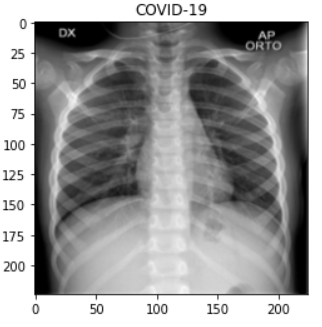
\includegraphics[scale=0.65]{./images/ejemploCOVID}
	\caption{Imagen de la clase COVID}
  \end{minipage}
  \hfill
  \begin{minipage}[b]{0.25\textwidth}
    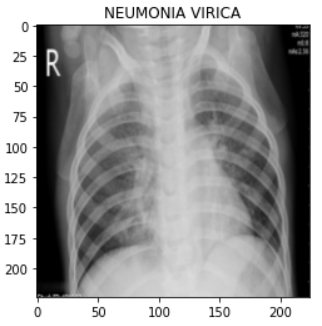
\includegraphics[scale=0.65]{./images/ejemploNEUMONIAVIRICA}
	\caption{Imagen de la clase Viral Pneumonia}
  \end{minipage}
    \hfill
    \begin{minipage}[b]{0.25\textwidth}
    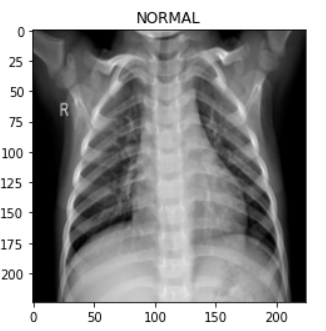
\includegraphics[scale=0.65]{./images/ejemploNORMAL}
	\caption{Imagen de la clase NORMAL}
  \end{minipage}
\end{figure}


\subsection{Creación de los conjuntos de train y test}

Primero creamos un vector agrupando las imágenes de las tres clases y cambiamos las etiquetas por números enteros, asignando el valor 0 a la clase COVID, el 1 a la clase NORMAL y el 2 a la clase Viral Pneumonia.\\

A continuación, usando la función \textit{to\_categorical} obtenemos una representación binaria de las clases (la clase 0 pasa a ser [1,0,0], la 1 es [0,1,0] y la 2 es [0,0,1]).\\

Ahora, para dividir los datos entre entrenamiento y test vamos a optar por hacer una permutación aleatoria de las imágenes, y posteriormente dividiéndolas en proporción 80\%-20\% para entrenamiento y test respectivamente, obteniendo un total de 2880 imágenes para entrenar y 720 para test. Hemos decidido hacer esta partición de los datos debido en parte a que, como hemos hecho notar antes, no hemos encontrado ninguna evidencia de que haya imágenes dentro del conjunto de datos que correspondan al mismo paciente en diferentes instantes de tiempo que puedan hacer que la tarea de clasificación se vea influenciada por este hecho. De ser así, que haya imágenes para un mismo paciente que cayeran unas en entrenamiento y otras en test, harían que aumentara el sobreajuste y la varianza de la red, haciendo que probablemente no generalizara bien y diera peores resultados en test. También pensamos que hubiera sido bastante útil hacer una división de los datos de forma temporal, dejando una proporción de las imágenes tomadas más recientemente como las imágenes para test, puesto que la enfermedad del COVID-19 está en constante evolución y buscamos que la red sea útil para poder ayudar a clasificar casos actuales de COVID-19 (aunque entendemos que las imágenes de pulmones sanos y pulmones con otros tipos de neumonías víricas no varían tanto a lo largo del tiempo). Sin embargo no hemos podido hacer esta división ya que no poseemos información de cuando se han tomado las imágenes. Son por estos hechos por los que hemos optado hacer el tipo de partición indicada.

\section{Implementación de los modelos}

En esta sección confeccionaremos distintos modelos convolucionales con distintas arquitecturas para poder compararlos y encontrar el que nos proporcione una mejor aproximación de solución a nuestro problema.\\

Principalmente nos hemos centrado en DenseNet121, que es el modelo inicial del que partimos, pero luego hemos probado otras arquitecturas similares partiendo de otros modelos conocidos para poder comparar.\\

Por último, también hemos probado con un modelo "from scratch", basado en la arquitectura diseñada por David en la práctica 2 para uno de los ejercicios, para comprobar cómo funciona este modelo, que no está preentrenado y es un poco más simple que los anteriores.\\

Para intentar que todos los modelos se entrenen en condiciones similares, hemos entrenado todos ellos durante 20 épocas.

\subsection{DenseNet121}

DenseNet121 es el modelo base que hemos elegido para empezar, puesto que es un modelo potente y entendemos que podríamos dar unos resultados decentes desde un primer momento aplicando técnicas sobre este modelo. En las primeras versiones vamos a utilizar el modelo, con los pesos de ImageNet, solo como extractor de características, a partir del cuál añadiremos modificaciones. Finalmente, haremos un ajuste fino del modelo donde sí moveremos los pesos.

\subsubsection{Version 0: Extractor de características inicial, sin entrenamiento}

Primero vamos a utilizar el modelo DenseNet121 preentrenado con IMAGENET sin entrenar ningún peso. Partiendo de las características extraídas, simplemente vamos a añadir la capa softmax y comprobaremos que los resultados no son para nada buenos, pues todavía no hemos entrenado nuevos pesos, no estamos adaptando la red a nuestros datos en absoluto.

Extraemos las características:

\begin{lstlisting}
#Vamos a cargar el modelo antes del ultimo pooling, para usarlo como extractor de caracteristicas
feat_extractor = DenseNet121(include_top=False, weights='imagenet', pooling='avg')
feat_extractor.trainable = False

#Una vez tenemos el modelo, vamos a compilarlo usando un optimizador y una funcion de perdida
opt = SGD(lr=0.01, decay= 1e-6, momentum=0.9, nesterov=True)

feat_extractor.compile(optimizer=opt, loss="categorical_crossentropy", metrics=["acc"])

#Con esto tenemos el modelo de densenet hasta que nos deja los datos en forma de vector unidimensional
#de dimension 1024
feat_extractor = keras.Model(inputs=feat_extractor.inputs, outputs= feat_extractor.layers[-1].output)

feat_extractor.compile(optimizer=opt, loss="categorical_crossentropy", metrics=["acc"])

# Extraer las caracteristicas de las imagenes con el modelo anterior.
car_train = feat_extractor.predict(x_train, verbose=1)
car_test = feat_extractor.predict(x_test, verbose=1)
\end{lstlisting}

El optimizador que he hemos empleado es el mismo que hemos usado en las prácticas, que es el que viene en las diapositivas, un gradiente descendente estocástico, con un tasa de aprendizaje de 0.01, con un paámetro de decaimiento de dicha tasa de aprendizaje de 1e-6, un momento de 0.9, y el descenso de gradiente se hará mediante la metodología Nesterov, en la cual, primero se realiza un desplazamiento en la dirección del gradiente acumulativo que llevamos, y posteriormente se realiza el nuevo cálculo del gradiente desde la posición en la que estemos en el espacio de búsqueda.\\

Una vez tenemos las características, añadimos la capa softmax y hacemos las predicciones.

\begin{lstlisting}
inputs = keras.layers.Input(shape=[1024])
outputs = keras.layers.Dense(units=3, activation="softmax")(inputs)

dense_model = keras.Model(inputs=inputs, outputs=outputs)
opt = SGD(lr=0.01, decay= 1e-6, momentum=0.9, nesterov=True)
dense_model.compile(optimizer=opt, loss="categorical_crossentropy", metrics=["acc"])

#Clasificamos
y_preds = dense_model.predict(car_test, verbose=True)

print("La accuracy del modelo es: " + str(calcularAccuracy(y_test, y_preds)))

y_test_conf = np.argmax(y_test, axis=1)
y_preds = np.argmax(y_preds, axis=1)
print("La matriz de confusion de las predicciones ha sido: \n", confusion_matrix(y_test_conf, y_preds))
\end{lstlisting}


Los resultados los podemos observar en la siguiente tabla:

\begin{table}[H]
\centering
\begin{tabular}{|c|c|c|c|c|c|c|}
\hline
\rowcolor[rgb]{0.753,0.753,0.753}  \textbf{Modelo}  & \textbf{Loss}                               & \textbf{Accuracy}                           & \begin{tabular}[c]{@{}>{\cellcolor[rgb]{0.753,0.753,0.753}}c@{}}\textbf{Validation}\\\textbf{ Loss} \end{tabular} & \begin{tabular}[c]{@{}>{\cellcolor[rgb]{0.753,0.753,0.753}}c@{}}\textbf{Validation }\\\textbf{ Accuracy} \end{tabular} & \begin{tabular}[c]{@{}>{\cellcolor[rgb]{0.753,0.753,0.753}}c@{}}\textbf{Test }\\\textbf{ Accuracy} \end{tabular} & \begin{tabular}[c]{@{}>{\cellcolor[rgb]{0.753,0.753,0.753}}c@{}}\textbf{Número}\\\textbf{Épocas} \end{tabular}  \\
\hline
\rowcolor[rgb]{0.937,0.937,0.937} DN-V0             &                                             &                                             &                                                                                                                   &                                                                                                                        & \textcolor[rgb]{0.129,0.129,0.129}{0.3264}                                                                       &                                                                                                                 \\
\hline

\end{tabular}
\caption{Resultados de la ejecución de la red DN-V0}
\end{table}

La matriz de confusión de la clasificación ha sido la siguiente:

\begin{table}[htpb]
\begin{center}
\begin{tabular}{l|
>{\columncolor[HTML]{EFEFEF}}l |
>{\columncolor[HTML]{EFEFEF}}l |
>{\columncolor[HTML]{EFEFEF}}l |}
\hline
\multicolumn{1}{|l|}{\cellcolor[HTML]{C0C0C0}\textbf{V-COVID}}  & 235                                      & 0                                         & 0                                       \\ \hline
\multicolumn{1}{|l|}{\cellcolor[HTML]{C0C0C0}\textbf{V-Normal}} & 244                                      & 0                                         & 0                                       \\ \hline
\multicolumn{1}{|l|}{\cellcolor[HTML]{C0C0C0}\textbf{V-Neum.}}  & 241                                      & 0                                         & 0                                       \\ \hline
                                                                & \cellcolor[HTML]{C0C0C0}\textbf{P-COVID} & \cellcolor[HTML]{C0C0C0}\textbf{P-Normal} & \cellcolor[HTML]{C0C0C0}\textbf{P-Neum} \\ \cline{2-4}
\end{tabular}
\end{center}
\caption{Matriz de confusión para la red DN-V0}
\end{table}

Podemos comprobar que efectivamente el modelo no es para nada satisfactorio. Obtenemos un valor de test accuracy cercano al 33\%, que sería justo lo equivalente a elegir una de las tres clases de forma aleatoria sin ningún tipo de criterio. De hecho, lo que hace es elegir la primera clase siempre de forma constante,  por lo que este modelo no tiene ningún tipo de utilidad ni interés. Se hace patente patente la necesidad de entrenar por lo menos la nueva capa de salida del modelo.

\subsubsection{Version 1: Extractor de características inicial, entrenando la capa de salida}

Ahora vamos a reentrenar sólo la capa de salida, sin ningún tratamiento adicional. La única diferencia respecto a la versión anterior es que sí que entrenamos la última capa:

\begin{lstlisting}
hist = dense_model.fit(car_train, y_train, batch_size=32, epochs=20, validation_split=0.1)
\end{lstlisting}

Los resultados obtenidos han sido los siguientes:

\begin{figure}[H]
  \centering
  \begin{minipage}[b]{0.45\textwidth}
    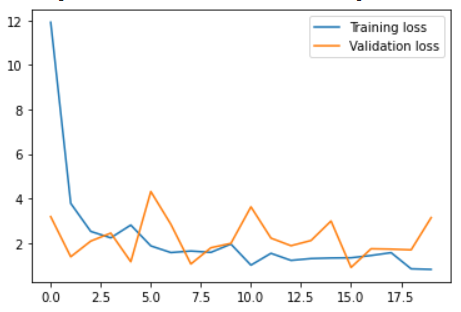
\includegraphics[scale=0.75]{./images/v1loss}
	\caption{Training-Validation Loss}
  \end{minipage}
  \hfill
  \begin{minipage}[b]{0.45\textwidth}
    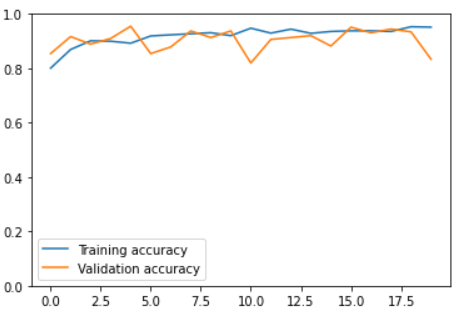
\includegraphics[scale=0.75]{./images/v1acc}
	\caption{Training-Validation accuracy}
  \end{minipage}
\end{figure}

\begin{table}[H]
\centering
\begin{tabular}{|c|c|c|c|c|c|c|}
\hline
\rowcolor[rgb]{0.753,0.753,0.753}  \textbf{Modelo}  & \textbf{Loss}                               & \textbf{Accuracy}                           & \begin{tabular}[c]{@{}>{\cellcolor[rgb]{0.753,0.753,0.753}}c@{}}\textbf{Validation}\\\textbf{ Loss} \end{tabular} & \begin{tabular}[c]{@{}>{\cellcolor[rgb]{0.753,0.753,0.753}}c@{}}\textbf{Validation }\\\textbf{ Accuracy} \end{tabular} & \begin{tabular}[c]{@{}>{\cellcolor[rgb]{0.753,0.753,0.753}}c@{}}\textbf{Test }\\\textbf{ Accuracy} \end{tabular} & \begin{tabular}[c]{@{}>{\cellcolor[rgb]{0.753,0.753,0.753}}c@{}}\textbf{Número}\\\textbf{Épocas} \end{tabular}  \\
\hline
\rowcolor[rgb]{0.937,0.937,0.937} DN-V0             &                                             &                                             &                                                                                                                   &                                                                                                                        & \textcolor[rgb]{0.129,0.129,0.129}{0.3264}                                                                       &                                                                                                                 \\
\hline
\rowcolor{green} DN-V1                                               & \textcolor[rgb]{0.129,0.129,0.129}{0.6501}  & \textcolor[rgb]{0.129,0.129,0.129}{0.9588 } & \textcolor[rgb]{0.129,0.129,0.129}{3.1393}                                                                        & \textcolor[rgb]{0.129,0.129,0.129}{0.8333}                                                                             & \textcolor[rgb]{0.129,0.129,0.129}{0.8361}                                                                       & 20                                                                                                              \\
\hline
\end{tabular}
\caption{Resultados de la ejecución para la red DN-V1, mostrando los anteriores}
\end{table}

\begin{table}[htbp]
\begin{center}
\begin{tabular}{l|
>{\columncolor[HTML]{EFEFEF}}l |
>{\columncolor[HTML]{EFEFEF}}l |
>{\columncolor[HTML]{EFEFEF}}l |}
\hline
\multicolumn{1}{|l|}{\cellcolor[HTML]{C0C0C0}\textbf{V-COVID}}  & 231                                      & 1                                         & 3                                       \\ \hline
\multicolumn{1}{|l|}{\cellcolor[HTML]{C0C0C0}\textbf{V-Normal}} & 6                                        & 135                                       & 103                                     \\ \hline
\multicolumn{1}{|l|}{\cellcolor[HTML]{C0C0C0}\textbf{V-Neum.}}  & 5                                        & 0                                         & 236                                     \\ \hline
                                                                & \cellcolor[HTML]{C0C0C0}\textbf{P-COVID} & \cellcolor[HTML]{C0C0C0}\textbf{P-Normal} & \cellcolor[HTML]{C0C0C0}\textbf{P-Neum} \\ \cline{2-4}
\end{tabular}
\end{center}
\caption{Matriz de confusión para la red DN-V1}
\end{table}

En este caso vemos que existe una notoria mejoría, consiguiendo unos resultados bastante buenos para solo haber incluido una capa final entrenable. Observando la matriz de confusión podemos apreciar que cuando predice que un pulmón es sano, tiene una tasa de acierto muy alta (tan solo un fallo), pero sin embargo tiene problemas con esta clase respecto a las demás neumonías víricas, pues hay 103 imágenes cuya predicción es Viral Pneumonia cuando realmente son pulmones sanos.

\subsubsection{Version 2: Data augmentation, más capas densas}

Seguimos empleando la red preentrenada como extractor de características pero se realiza un preprocesado más exhaustivo de imágenes, con image augmentation y normalización, además de hacer un modelo denso de mayor profundidad.\\

Además de hacer una normalización de las imágenes, para que tengan media cero y varianza 1, hemos detectado que hay imágenes que salen muy blancas y otras muy oscuras, luego debemos conseguir invarianza frente al brillo (añadiendo el parámetro brightness).\\

En cuanto al data augmentation, los pulmones en las radiografías salen siempre verticales, por lo que no tiene mucho sentido añadir rotaciones pero sí flips horizontales. Los zooms de ampliación también pueden ser interesantes, puesto que las imágenes tienen siempre los pulmones en la zona central, y podemos evitar posibles fuentes de ruido de letras o huesos que tienen algunas de las imágenes en las zonas laterales, que se perderán haciendo zoom.\\

Para aplicar todo esto, creamos un objeto de la clase ImageDataGenerator:

\begin{lstlisting}
#Image data generators

train_generator = ImageDataGenerator(featurewise_center = True,
                             featurewise_std_normalization = True,
                             validation_split=0.1,
                             horizontal_flip=True,
                             brightness_range=[0.8,1.25],
                             zoom_range=[1,1.2])
train_generator.fit(x_train)

test_generator = ImageDataGenerator(featurewise_center = True,
                             featurewise_std_normalization = True)

test_generator.fit(x_train)

it = train_generator.flow(x_train, batch_size=1)
\end{lstlisting}

Añadimos también alguna capa densa más para ganar profundidad:

\begin{lstlisting}
inputs = keras.layers.Input(shape=[1024])
layer1 = keras.layers.Dense(units=500, activation="relu")(inputs)
layer2 = keras.layers.Dense(units=200, activation="relu")(layer1)
outputs = keras.layers.Dense(units=3, activation="softmax")(layer2)
\end{lstlisting}

Entrenamos el modelo obteniendo los siguientes resultados:

\begin{figure}[H]
  \centering
  \begin{minipage}[b]{0.45\textwidth}
    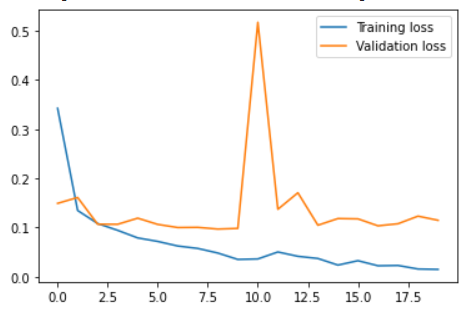
\includegraphics[scale=0.75]{./images/v2loss}
	\caption{Training-Validation Loss}
  \end{minipage}
  \hfill
  \begin{minipage}[b]{0.45\textwidth}
    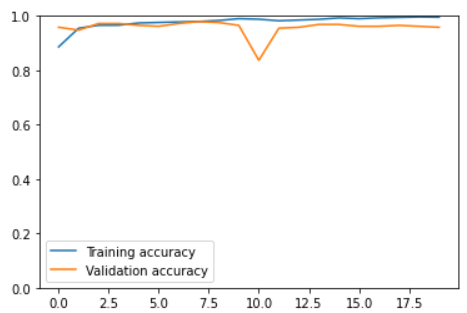
\includegraphics[scale=0.75]{./images/v2acc}
	\caption{Training-Validation accuracy}
  \end{minipage}
\end{figure}

\begin{table}[H]
\centering
\begin{tabular}{|c|c|c|c|c|c|c|}
\hline
\rowcolor[rgb]{0.753,0.753,0.753}  \textbf{Modelo}  & \textbf{Loss}                               & \textbf{Accuracy}                           & \begin{tabular}[c]{@{}>{\cellcolor[rgb]{0.753,0.753,0.753}}c@{}}\textbf{Validation}\\\textbf{ Loss} \end{tabular} & \begin{tabular}[c]{@{}>{\cellcolor[rgb]{0.753,0.753,0.753}}c@{}}\textbf{Validation }\\\textbf{ Accuracy} \end{tabular} & \begin{tabular}[c]{@{}>{\cellcolor[rgb]{0.753,0.753,0.753}}c@{}}\textbf{Test }\\\textbf{ Accuracy} \end{tabular} & \begin{tabular}[c]{@{}>{\cellcolor[rgb]{0.753,0.753,0.753}}c@{}}\textbf{Número}\\\textbf{Épocas} \end{tabular}  \\
\hline
\rowcolor[rgb]{0.937,0.937,0.937} DN-V0             &                                             &                                             &                                                                                                                   &                                                                                                                        & \textcolor[rgb]{0.129,0.129,0.129}{0.3264}                                                                       &                                                                                                                 \\
\hline
DN-V1                                               & \textcolor[rgb]{0.129,0.129,0.129}{0.6501}  & \textcolor[rgb]{0.129,0.129,0.129}{0.9588 } & \textcolor[rgb]{0.129,0.129,0.129}{3.1393}                                                                        & \textcolor[rgb]{0.129,0.129,0.129}{0.8333}                                                                             & \textcolor[rgb]{0.129,0.129,0.129}{0.8361}                                                                       & 20                                                                                                              \\
\hline
\rowcolor{green} DN-V2                                               & \textcolor[rgb]{0.129,0.129,0.129}{0.0109 } & \textcolor[rgb]{0.129,0.129,0.129}{0.9973 } & \textcolor[rgb]{0.129,0.129,0.129}{0.1146 }                                                                       & \textcolor[rgb]{0.129,0.129,0.129}{0.9583}                                                                             & \textcolor[rgb]{0.129,0.129,0.129}{0.9597}                                                                       & 20                                                                                                              \\
\hline


\end{tabular}
\caption{Resultados de la ejecución para la red DN-V2, mostrando los anteriores}
\end{table}


\begin{table}[htbp]
\begin{center}
\begin{tabular}{l|
>{\columncolor[HTML]{EFEFEF}}l |
>{\columncolor[HTML]{EFEFEF}}l |
>{\columncolor[HTML]{EFEFEF}}l |}
\hline
\multicolumn{1}{|l|}{\cellcolor[HTML]{C0C0C0}\textbf{V-COVID}}  & 230                                      & 3                                         & 2                                       \\ \hline
\multicolumn{1}{|l|}{\cellcolor[HTML]{C0C0C0}\textbf{V-Normal}} & 1                                        & 238                                       & 5                                       \\ \hline
\multicolumn{1}{|l|}{\cellcolor[HTML]{C0C0C0}\textbf{V-Neum.}}  & 1                                        & 17                                        & 223                                     \\ \hline
                                                                & \cellcolor[HTML]{C0C0C0}\textbf{P-COVID} & \cellcolor[HTML]{C0C0C0}\textbf{P-Normal} & \cellcolor[HTML]{C0C0C0}\textbf{P-Neum} \\ \cline{2-4}
\end{tabular}
\end{center}
\caption{Matriz de confusión para la red DN-V2}
\end{table}



Podemos ver que la mejora ha sido bastante efectiva, obteniendo un valor para test accuracy de 0.9597. Sin embargo, si nos fijamos en las gráficas, puede ser que tengamos un poco de overfitting puesto que el validation loss no decrece al mismo ritmo que el training loss.  Además hay un enorme pico tanto en la función de pérdida como en el accuracy de la validación, lo que también nos hace sospechar que es debido a un overfitting.\\

Para solucionar esto, regularizamos el modelo añadiendo una capa de Dropout.

\begin{lstlisting}
inputs = keras.layers.Input(shape=[1024])
layer1 = keras.layers.Dense(units=500, activation="relu")(inputs)
layer2 = keras.layers.Dropout(0.5)(layer1)
layer3 = keras.layers.Dense(units=200, activation="relu")(layer2)
outputs = keras.layers.Dense(units=3, activation="softmax")(layer3)
\end{lstlisting}

\begin{figure}[H]
  \centering
  \begin{minipage}[b]{0.45\textwidth}
    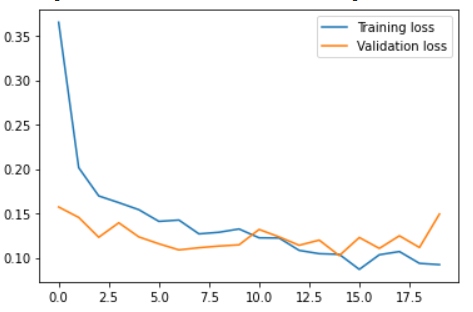
\includegraphics[scale=0.75]{./images/v2-2loss}
	\caption{Training-Validation Loss}
  \end{minipage}
  \hfill
  \begin{minipage}[b]{0.45\textwidth}
    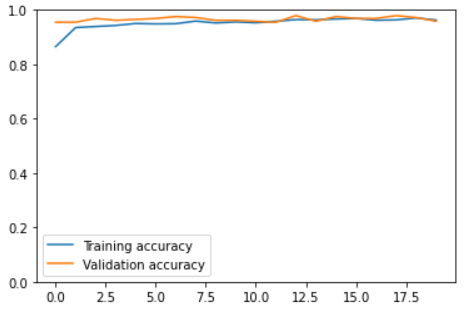
\includegraphics[scale=0.75]{./images/v2-2acc}
	\caption{Training-Validation accuracy}
  \end{minipage}
\end{figure}

\begin{table}[H]
\centering
\begin{tabular}{|c|c|c|c|c|c|c|}
\hline
\rowcolor[rgb]{0.753,0.753,0.753}  \textbf{Modelo}  & \textbf{Loss}                               & \textbf{Accuracy}                           & \begin{tabular}[c]{@{}>{\cellcolor[rgb]{0.753,0.753,0.753}}c@{}}\textbf{Validation}\\\textbf{ Loss} \end{tabular} & \begin{tabular}[c]{@{}>{\cellcolor[rgb]{0.753,0.753,0.753}}c@{}}\textbf{Validation }\\\textbf{ Accuracy} \end{tabular} & \begin{tabular}[c]{@{}>{\cellcolor[rgb]{0.753,0.753,0.753}}c@{}}\textbf{Test }\\\textbf{ Accuracy} \end{tabular} & \begin{tabular}[c]{@{}>{\cellcolor[rgb]{0.753,0.753,0.753}}c@{}}\textbf{Número}\\\textbf{Épocas} \end{tabular}  \\
\hline
\rowcolor[rgb]{0.937,0.937,0.937} DN-V0             &                                             &                                             &                                                                                                                   &                                                                                                                        & \textcolor[rgb]{0.129,0.129,0.129}{0.3264}                                                                       &                                                                                                                 \\
\hline
DN-V1                                               & \textcolor[rgb]{0.129,0.129,0.129}{0.6501}  & \textcolor[rgb]{0.129,0.129,0.129}{0.9588 } & \textcolor[rgb]{0.129,0.129,0.129}{3.1393}                                                                        & \textcolor[rgb]{0.129,0.129,0.129}{0.8333}                                                                             & \textcolor[rgb]{0.129,0.129,0.129}{0.8361}                                                                       & 20                                                                                                              \\
\hline
DN-V2                                               & \textcolor[rgb]{0.129,0.129,0.129}{0.0109 } & \textcolor[rgb]{0.129,0.129,0.129}{0.9973 } & \textcolor[rgb]{0.129,0.129,0.129}{0.1146 }                                                                       & \textcolor[rgb]{0.129,0.129,0.129}{0.9583}                                                                             & \textcolor[rgb]{0.129,0.129,0.129}{0.9597}                                                                       & 20                                                                                                              \\
\hline
\rowcolor{green} DN-V2-reg                                           & \textcolor[rgb]{0.129,0.129,0.129}{0.0883 } & \textcolor[rgb]{0.129,0.129,0.129}{0.9683 } & \textcolor[rgb]{0.129,0.129,0.129}{0.1494 }                                                                       & \textcolor[rgb]{0.129,0.129,0.129}{0.9583}                                                                             & \textcolor[rgb]{0.129,0.129,0.129}{0.9569}                                                                       & 20                                                                                                              \\
\hline

\end{tabular}
\caption{Resultados de la ejecución para la red DN-V2-reg mostrando los anteriores}
\end{table}

\begin{table}[htbp]
\begin{center}
\begin{tabular}{l|
>{\columncolor[HTML]{EFEFEF}}l |
>{\columncolor[HTML]{EFEFEF}}l |
>{\columncolor[HTML]{EFEFEF}}l |}
\hline
\multicolumn{1}{|l|}{\cellcolor[HTML]{C0C0C0}\textbf{V-COVID}}  & 226                                      & 2                                         & 7                                       \\ \hline
\multicolumn{1}{|l|}{\cellcolor[HTML]{C0C0C0}\textbf{V-Normal}} & 0                                        & 233                                       & 11                                      \\ \hline
\multicolumn{1}{|l|}{\cellcolor[HTML]{C0C0C0}\textbf{V-Neum.}}  & 0                                        & 11                                        & 230                                     \\ \hline
                                                                & \cellcolor[HTML]{C0C0C0}\textbf{P-COVID} & \cellcolor[HTML]{C0C0C0}\textbf{P-Normal} & \cellcolor[HTML]{C0C0C0}\textbf{P-Neum} \\ \cline{2-4}
\end{tabular}
\end{center}
\caption{Matriz de confusión para la red DN-V2-reg}
\end{table}

Con la regularización hemos conseguido mantener prácticamente la precisión que teníamos, pero hemos reducido un poco el overfitting que había, como podemos comprobar en las gráficas.  Como hemos visto ya no hay ningún salto brusco y durante todo el entrenamiento se produce una evolución más estable, y la función de pérdida de validación parece no decrecer porque si nos fijamos en el gráfico del accuracy ya se ha alcanzado un punto de estabilidad muy alto para validación.\\

Comparando la matriz de confusión con la primera que comentamos, vemos que se ha mejorado el problema que había (las 103 imágenes clasificadas como Viral Pneumonia cuando eran pulmones sanos han pasado a ser solo 11). Otro aspecto a comentar es que la clase que mejor clasifica es la clase COVID, con solo 9 ejemplos mal clasificados, con respecto a los 11 ejemplos mal clasificados de las otras 2 clases.

\subsubsection{Version 3: Fine tunning}

Vamos a probar ahora a hacer un ajuste fino de la red completa, tomando como pesos iniciales los de imagenet. Ahora ya no solo vamos a utilizar DenseNet como extractor de características, sino que, en vez de estar la red congelada, vamos a ir moviendo sus pesos con el entrenamiento. Esto permitirá a la red entera adaptarse al conjunto de entrenamiento, y ya no consideraremos la parte convolucional como un extractor de características estático, como sí lo era antes.\\

En este caso, indicamos que los pesos sí son entrenables:

\begin{lstlisting}
denseNet.trainable = True
\end{lstlisting}

Entrenamos con la función \textit{fit\_generator} y obtenemos lo siguiente:

\begin{figure}[H]
  \centering
  \begin{minipage}[b]{0.45\textwidth}
    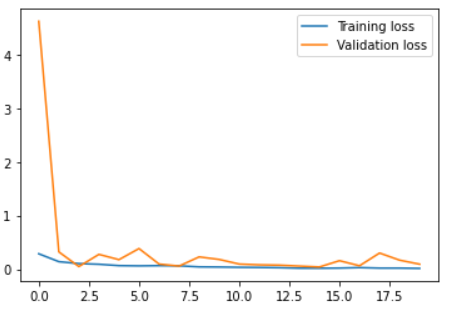
\includegraphics[scale=0.75]{./images/v3loss}
	\caption{Training-Validation Loss}
  \end{minipage}
  \hfill
  \begin{minipage}[b]{0.45\textwidth}
    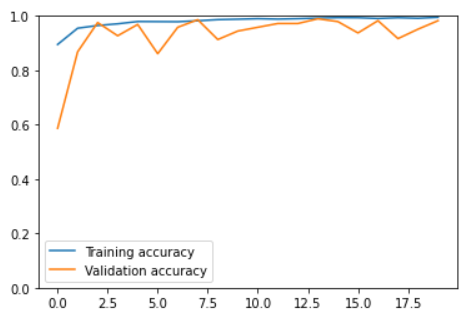
\includegraphics[scale=0.75]{./images/v3acc}
	\caption{Training-Validation accuracy}
  \end{minipage}
\end{figure}

\begin{table}[H]
\centering
\begin{tabular}{|c|c|c|c|c|c|c|}
\hline
\rowcolor[rgb]{0.753,0.753,0.753}  \textbf{Modelo}  & \textbf{Loss}                               & \textbf{Accuracy}                           & \begin{tabular}[c]{@{}>{\cellcolor[rgb]{0.753,0.753,0.753}}c@{}}\textbf{Validation}\\\textbf{ Loss} \end{tabular} & \begin{tabular}[c]{@{}>{\cellcolor[rgb]{0.753,0.753,0.753}}c@{}}\textbf{Validation }\\\textbf{ Accuracy} \end{tabular} & \begin{tabular}[c]{@{}>{\cellcolor[rgb]{0.753,0.753,0.753}}c@{}}\textbf{Test }\\\textbf{ Accuracy} \end{tabular} & \begin{tabular}[c]{@{}>{\cellcolor[rgb]{0.753,0.753,0.753}}c@{}}\textbf{Número}\\\textbf{Épocas} \end{tabular}  \\
\hline
\rowcolor[rgb]{0.937,0.937,0.937} DN-V0             &                                             &                                             &                                                                                                                   &                                                                                                                        & \textcolor[rgb]{0.129,0.129,0.129}{0.3264}                                                                       &                                                                                                                 \\
\hline
DN-V1                                               & \textcolor[rgb]{0.129,0.129,0.129}{0.6501}  & \textcolor[rgb]{0.129,0.129,0.129}{0.9588 } & \textcolor[rgb]{0.129,0.129,0.129}{3.1393}                                                                        & \textcolor[rgb]{0.129,0.129,0.129}{0.8333}                                                                             & \textcolor[rgb]{0.129,0.129,0.129}{0.8361}                                                                       & 20                                                                                                              \\
\hline
DN-V2                                               & \textcolor[rgb]{0.129,0.129,0.129}{0.0109 } & \textcolor[rgb]{0.129,0.129,0.129}{0.9973 } & \textcolor[rgb]{0.129,0.129,0.129}{0.1146 }                                                                       & \textcolor[rgb]{0.129,0.129,0.129}{0.9583}                                                                             & \textcolor[rgb]{0.129,0.129,0.129}{0.9597}                                                                       & 20                                                                                                              \\
\hline
DN-V2-reg                                           & \textcolor[rgb]{0.129,0.129,0.129}{0.0883 } & \textcolor[rgb]{0.129,0.129,0.129}{0.9683 } & \textcolor[rgb]{0.129,0.129,0.129}{0.1494 }                                                                       & \textcolor[rgb]{0.129,0.129,0.129}{0.9583}                                                                             & \textcolor[rgb]{0.129,0.129,0.129}{0.9569}                                                                       & 20                                                                                                              \\
\hline
\rowcolor{green} DN-V3                                               & \textcolor[rgb]{0.129,0.129,0.129}{0.0089 } & \textcolor[rgb]{0.129,0.129,0.129}{0.9964 } & \textcolor[rgb]{0.129,0.129,0.129}{0.0924 }                                                                       & \textcolor[rgb]{0.129,0.129,0.129}{0.9826}                                                                             & \textcolor[rgb]{0.129,0.129,0.129}{0.9736}                                                                       & 20                                                                                                              \\
\hline


\end{tabular}
\caption{Resultados de la ejecución para la red DN-V3, mostrando los anteriores}
\end{table}

\begin{table}[htbp]
\begin{center}
\begin{tabular}{l|
>{\columncolor[HTML]{EFEFEF}}l |
>{\columncolor[HTML]{EFEFEF}}l |
>{\columncolor[HTML]{EFEFEF}}l |}
\hline
\multicolumn{1}{|l|}{\cellcolor[HTML]{C0C0C0}\textbf{V-COVID}}  & 235                                      & 0                                         & 0                                       \\ \hline
\multicolumn{1}{|l|}{\cellcolor[HTML]{C0C0C0}\textbf{V-Normal}} & 0                                        & 230                                       & 14                                      \\ \hline
\multicolumn{1}{|l|}{\cellcolor[HTML]{C0C0C0}\textbf{V-Neum.}}  & 4                                        & 1                                         & 236                                     \\ \hline
                                                                & \cellcolor[HTML]{C0C0C0}\textbf{P-COVID} & \cellcolor[HTML]{C0C0C0}\textbf{P-Normal} & \cellcolor[HTML]{C0C0C0}\textbf{P-Neum} \\ \cline{2-4}
\end{tabular}
\end{center}
\caption{Matriz de confusión para la red DN-V3}
\end{table}

Los resultados obtenidos son bastante buenos, superando el 97\% de test accuracy. La matriz de confusión nos sigue indicando que el único pequeño problema que sigue teniendo son esas 14 imágenes de la clase NORMAL clasificadas como Viral Pneumonia, que aunque se ha reducido respecto a las versiones iniciales, ha sido notable en todos los modelos.\\

\subsubsection{Modificaciones a aplicar a las siguientes redes}

Ahora vamos a aplicar las siguientes modificaciones que hemos empleado en estas versiones a distintas arquitecturas distintas a DenseNetet121.
\begin{itemize}
\item El esquema de modificaciones de la versión 2, donde utilizábamos la red inicial como extractor de características constante,  entrenando un pequeño modelo denso al final y utilizando el data augmentation que hemos visto. Notaremos a las redes con estas modificaciones con el nombre de la red base, seguido de EC (Extractor de Características)
\item El esquema de modificacionesde la versión 3, donde utilizábamos un ajuste fino, empleando también el mismo data augmentation. Notaremos a las redes con estas modificaciones con el nombre de la red base, seguido de FT (Fine Tunning)
\end{itemize}

Evidentemente todas las redes que usemos serán redes preentrenadas con los pesos de su entrenamiento con el challenge de Imagenet.


\subsection{ResNet50}

\subsubsection{ResNet-EC}

\begin{figure}[H]
  \centering
  \begin{minipage}[b]{0.45\textwidth}
    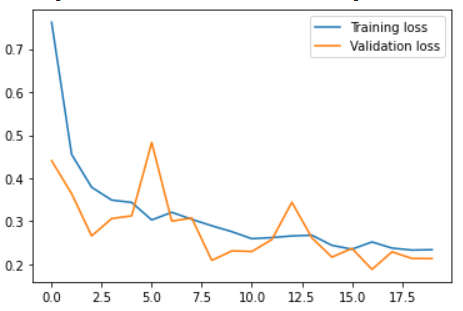
\includegraphics[scale=0.75]{./images/resnet1loss}
	\caption{Training-Validation Loss}
  \end{minipage}
  \hfill
  \begin{minipage}[b]{0.45\textwidth}
    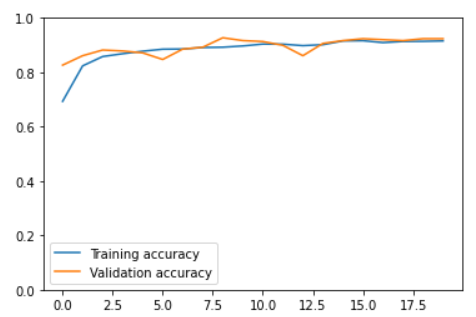
\includegraphics[scale=0.75]{./images/resnet1acc}
	\caption{Training-Validation accuracy}
  \end{minipage}
\end{figure}



\begin{table}[H]
\centering
\begin{tabular}{|c|c|c|c|c|c|c|}
\hline
\rowcolor[rgb]{0.753,0.753,0.753}  \textbf{Modelo}  & \textbf{Loss}                               & \textbf{Accuracy}                           & \begin{tabular}[c]{@{}>{\cellcolor[rgb]{0.753,0.753,0.753}}c@{}}\textbf{Validation}\\\textbf{ Loss} \end{tabular} & \begin{tabular}[c]{@{}>{\cellcolor[rgb]{0.753,0.753,0.753}}c@{}}\textbf{Validation }\\\textbf{ Accuracy} \end{tabular} & \begin{tabular}[c]{@{}>{\cellcolor[rgb]{0.753,0.753,0.753}}c@{}}\textbf{Test }\\\textbf{ Accuracy} \end{tabular} & \begin{tabular}[c]{@{}>{\cellcolor[rgb]{0.753,0.753,0.753}}c@{}}\textbf{Número}\\\textbf{Épocas} \end{tabular}  \\
\hline
\rowcolor[rgb]{0.937,0.937,0.937} DN-V0             &                                             &                                             &                                                                                                                   &                                                                                                                        & \textcolor[rgb]{0.129,0.129,0.129}{0.3264}                                                                       &                                                                                                                 \\
\hline
DN-V1                                               & \textcolor[rgb]{0.129,0.129,0.129}{0.6501}  & \textcolor[rgb]{0.129,0.129,0.129}{0.9588 } & \textcolor[rgb]{0.129,0.129,0.129}{3.1393}                                                                        & \textcolor[rgb]{0.129,0.129,0.129}{0.8333}                                                                             & \textcolor[rgb]{0.129,0.129,0.129}{0.8361}                                                                       & 20                                                                                                              \\
\hline
DN-V2                                               & \textcolor[rgb]{0.129,0.129,0.129}{0.0109 } & \textcolor[rgb]{0.129,0.129,0.129}{0.9973 } & \textcolor[rgb]{0.129,0.129,0.129}{0.1146 }                                                                       & \textcolor[rgb]{0.129,0.129,0.129}{0.9583}                                                                             & \textcolor[rgb]{0.129,0.129,0.129}{0.9597}                                                                       & 20                                                                                                              \\
\hline
DN-V2-reg                                           & \textcolor[rgb]{0.129,0.129,0.129}{0.0883 } & \textcolor[rgb]{0.129,0.129,0.129}{0.9683 } & \textcolor[rgb]{0.129,0.129,0.129}{0.1494 }                                                                       & \textcolor[rgb]{0.129,0.129,0.129}{0.9583}                                                                             & \textcolor[rgb]{0.129,0.129,0.129}{0.9569}                                                                       & 20                                                                                                              \\
\hline
DN-V3                                               & \textcolor[rgb]{0.129,0.129,0.129}{0.0089 } & \textcolor[rgb]{0.129,0.129,0.129}{0.9964 } & \textcolor[rgb]{0.129,0.129,0.129}{0.0924 }                                                                       & \textcolor[rgb]{0.129,0.129,0.129}{0.9826}                                                                             & \textcolor[rgb]{0.129,0.129,0.129}{0.9736}                                                                       & 20                                                                                                              \\
\hline
\rowcolor{green} ResNet-EC                                              & \textcolor[rgb]{0.129,0.129,0.129}{0.2519 } & \textcolor[rgb]{0.129,0.129,0.129}{0.9063 } & \textcolor[rgb]{0.129,0.129,0.129}{0.2134 }                                                                       & \textcolor[rgb]{0.129,0.129,0.129}{0.9236}                                                                             & \textcolor[rgb]{0.129,0.129,0.129}{0.8805}                                                                       & 20                                                                                                              \\
\hline


\end{tabular}
\caption{Resultados de la ejecución para la red ResNet-EC, mostrando los anteriores}
\end{table}


\begin{table}[htbp]
\begin{center}
\begin{tabular}{l|
>{\columncolor[HTML]{EFEFEF}}l |
>{\columncolor[HTML]{EFEFEF}}l |
>{\columncolor[HTML]{EFEFEF}}l |}
\hline
\multicolumn{1}{|l|}{\cellcolor[HTML]{C0C0C0}\textbf{V-COVID}}  & 234                                      & 1                                         & 0                                       \\ \hline
\multicolumn{1}{|l|}{\cellcolor[HTML]{C0C0C0}\textbf{V-Normal}} & 15                                       & 219                                       & 10                                      \\ \hline
\multicolumn{1}{|l|}{\cellcolor[HTML]{C0C0C0}\textbf{V-Neum.}}  & 46                                       & 14                                        & 181                                     \\ \hline
                                                                & \cellcolor[HTML]{C0C0C0}\textbf{P-COVID} & \cellcolor[HTML]{C0C0C0}\textbf{P-Normal} & \cellcolor[HTML]{C0C0C0}\textbf{P-Neum} \\ \cline{2-4}
\end{tabular}
\end{center}
\caption{Matriz de confusión para la red ResNet-EC}
\end{table}


El resultado obtenido no es malo, pero tampoco se acerca al anterior de DenseNet en su versión homóloga. \\

\subsubsection{ResNet-FT}
Para la versión fine tunning:

\begin{figure}[H]
  \centering
  \begin{minipage}[b]{0.45\textwidth}
    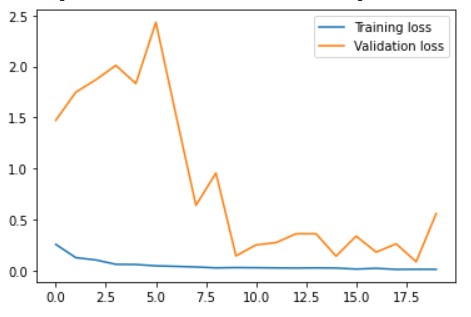
\includegraphics[scale=0.75]{./images/resnet2loss}
	\caption{Training-Validation Loss}
  \end{minipage}
  \hfill
  \begin{minipage}[b]{0.45\textwidth}
    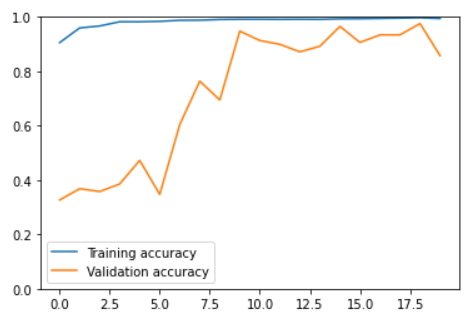
\includegraphics[scale=0.75]{./images/resnet2acc}
	\caption{Training-Validation accuracy}
  \end{minipage}
\end{figure}

\begin{table}[H]
\centering
\begin{tabular}{|c|c|c|c|c|c|c|}
\hline
\rowcolor[rgb]{0.753,0.753,0.753}  \textbf{Modelo}  & \textbf{Loss}                               & \textbf{Accuracy}                           & \begin{tabular}[c]{@{}>{\cellcolor[rgb]{0.753,0.753,0.753}}c@{}}\textbf{Validation}\\\textbf{ Loss} \end{tabular} & \begin{tabular}[c]{@{}>{\cellcolor[rgb]{0.753,0.753,0.753}}c@{}}\textbf{Validation }\\\textbf{ Accuracy} \end{tabular} & \begin{tabular}[c]{@{}>{\cellcolor[rgb]{0.753,0.753,0.753}}c@{}}\textbf{Test }\\\textbf{ Accuracy} \end{tabular} & \begin{tabular}[c]{@{}>{\cellcolor[rgb]{0.753,0.753,0.753}}c@{}}\textbf{Número}\\\textbf{Épocas} \end{tabular}  \\
\hline
\rowcolor[rgb]{0.937,0.937,0.937} DN-V0             &                                             &                                             &                                                                                                                   &                                                                                                                        & \textcolor[rgb]{0.129,0.129,0.129}{0.3264}                                                                       &                                                                                                                 \\
\hline
DN-V1                                               & \textcolor[rgb]{0.129,0.129,0.129}{0.6501}  & \textcolor[rgb]{0.129,0.129,0.129}{0.9588 } & \textcolor[rgb]{0.129,0.129,0.129}{3.1393}                                                                        & \textcolor[rgb]{0.129,0.129,0.129}{0.8333}                                                                             & \textcolor[rgb]{0.129,0.129,0.129}{0.8361}                                                                       & 20                                                                                                              \\
\hline
DN-V2                                               & \textcolor[rgb]{0.129,0.129,0.129}{0.0109 } & \textcolor[rgb]{0.129,0.129,0.129}{0.9973 } & \textcolor[rgb]{0.129,0.129,0.129}{0.1146 }                                                                       & \textcolor[rgb]{0.129,0.129,0.129}{0.9583}                                                                             & \textcolor[rgb]{0.129,0.129,0.129}{0.9597}                                                                       & 20                                                                                                              \\
\hline
DN-V2-reg                                           & \textcolor[rgb]{0.129,0.129,0.129}{0.0883 } & \textcolor[rgb]{0.129,0.129,0.129}{0.9683 } & \textcolor[rgb]{0.129,0.129,0.129}{0.1494 }                                                                       & \textcolor[rgb]{0.129,0.129,0.129}{0.9583}                                                                             & \textcolor[rgb]{0.129,0.129,0.129}{0.9569}                                                                       & 20                                                                                                              \\
\hline
DN-V3                                               & \textcolor[rgb]{0.129,0.129,0.129}{0.0089 } & \textcolor[rgb]{0.129,0.129,0.129}{0.9964 } & \textcolor[rgb]{0.129,0.129,0.129}{0.0924 }                                                                       & \textcolor[rgb]{0.129,0.129,0.129}{0.9826}                                                                             & \textcolor[rgb]{0.129,0.129,0.129}{0.9736}                                                                       & 20                                                                                                              \\
\hline
ResNet-EC                                              & \textcolor[rgb]{0.129,0.129,0.129}{0.2519 } & \textcolor[rgb]{0.129,0.129,0.129}{0.9063 } & \textcolor[rgb]{0.129,0.129,0.129}{0.2134 }                                                                       & \textcolor[rgb]{0.129,0.129,0.129}{0.9236}                                                                             & \textcolor[rgb]{0.129,0.129,0.129}{0.8805}                                                                       & 20                                                                                                              \\
\hline
\rowcolor{green} ResNet-FT                                           & \textcolor[rgb]{0.129,0.129,0.129}{0.0102 } & \textcolor[rgb]{0.129,0.129,0.129}{0.9952 } & \textcolor[rgb]{0.129,0.129,0.129}{0.5594 }                                                                       & \textcolor[rgb]{0.129,0.129,0.129}{0.8576}                                                                             & \textcolor[rgb]{0.129,0.129,0.129}{0.8736}                                                                       & 20                                                                                                              \\
\hline


\end{tabular}

\caption{Resultados de la ejecución para la red ResNet-FT, mostrando los anteriores}
\end{table}


\begin{table}[htbp]
\begin{center}
\begin{tabular}{l|
>{\columncolor[HTML]{EFEFEF}}l |
>{\columncolor[HTML]{EFEFEF}}l |
>{\columncolor[HTML]{EFEFEF}}l |}
\hline
\multicolumn{1}{|l|}{\cellcolor[HTML]{C0C0C0}\textbf{V-COVID}}  & 173                                      & 0                                         & 62                                      \\ \hline
\multicolumn{1}{|l|}{\cellcolor[HTML]{C0C0C0}\textbf{V-Normal}} & 2                                        & 220                                       & 22                                      \\ \hline
\multicolumn{1}{|l|}{\cellcolor[HTML]{C0C0C0}\textbf{V-Neum.}}  & 0                                        & 5                                         & 236                                     \\ \hline
                                                                & \cellcolor[HTML]{C0C0C0}\textbf{P-COVID} & \cellcolor[HTML]{C0C0C0}\textbf{P-Normal} & \cellcolor[HTML]{C0C0C0}\textbf{P-Neum} \\ \cline{2-4}
\end{tabular}
\end{center}
\caption{Matriz de confusión para la red ResNet-FT}
\end{table}

A diferencia de lo que pasaba con DenseNet, con ResNet no ha funcionado mejor hacer fine tunning. Además, por las gráficas podemos apreciar que tal y como hemos definido la arquitectura tenemos overfitting, por lo que tendríamos que regularizarlo aún más para mejorar el aprendizaje. 

\subsection{VGG16}

\subsubsection{VGG16-EC}

\begin{figure}[H]
  \centering
  \begin{minipage}[b]{0.45\textwidth}
    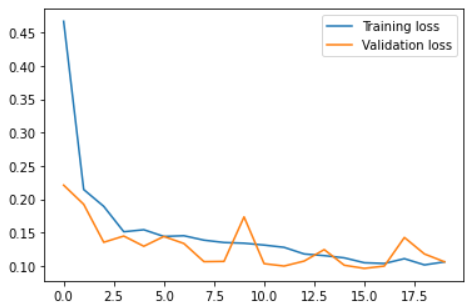
\includegraphics[scale=0.75]{./images/vggloss}
	\caption{Training-Validation Loss}
  \end{minipage}
  \hfill
  \begin{minipage}[b]{0.45\textwidth}
    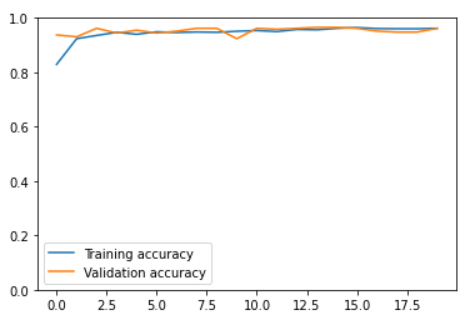
\includegraphics[scale=0.75]{./images/vggacc}
	\caption{Training-Validation accuracy}
  \end{minipage}
\end{figure}

\begin{table}[H]
\centering
\begin{tabular}{|c|c|c|c|c|c|c|}
\hline
\rowcolor[rgb]{0.753,0.753,0.753}  \textbf{Modelo}  & \textbf{Loss}                               & \textbf{Accuracy}                           & \begin{tabular}[c]{@{}>{\cellcolor[rgb]{0.753,0.753,0.753}}c@{}}\textbf{Validation}\\\textbf{ Loss} \end{tabular} & \begin{tabular}[c]{@{}>{\cellcolor[rgb]{0.753,0.753,0.753}}c@{}}\textbf{Validation }\\\textbf{ Accuracy} \end{tabular} & \begin{tabular}[c]{@{}>{\cellcolor[rgb]{0.753,0.753,0.753}}c@{}}\textbf{Test }\\\textbf{ Accuracy} \end{tabular} & \begin{tabular}[c]{@{}>{\cellcolor[rgb]{0.753,0.753,0.753}}c@{}}\textbf{Número}\\\textbf{Épocas} \end{tabular}  \\
\hline
\rowcolor[rgb]{0.937,0.937,0.937} DN-V0             &                                             &                                             &                                                                                                                   &                                                                                                                        & \textcolor[rgb]{0.129,0.129,0.129}{0.3264}                                                                       &                                                                                                                 \\
\hline
DN-V1                                               & \textcolor[rgb]{0.129,0.129,0.129}{0.6501}  & \textcolor[rgb]{0.129,0.129,0.129}{0.9588 } & \textcolor[rgb]{0.129,0.129,0.129}{3.1393}                                                                        & \textcolor[rgb]{0.129,0.129,0.129}{0.8333}                                                                             & \textcolor[rgb]{0.129,0.129,0.129}{0.8361}                                                                       & 20                                                                                                              \\
\hline
DN-V2                                               & \textcolor[rgb]{0.129,0.129,0.129}{0.0109 } & \textcolor[rgb]{0.129,0.129,0.129}{0.9973 } & \textcolor[rgb]{0.129,0.129,0.129}{0.1146 }                                                                       & \textcolor[rgb]{0.129,0.129,0.129}{0.9583}                                                                             & \textcolor[rgb]{0.129,0.129,0.129}{0.9597}                                                                       & 20                                                                                                              \\
\hline
DN-V2-reg                                           & \textcolor[rgb]{0.129,0.129,0.129}{0.0883 } & \textcolor[rgb]{0.129,0.129,0.129}{0.9683 } & \textcolor[rgb]{0.129,0.129,0.129}{0.1494 }                                                                       & \textcolor[rgb]{0.129,0.129,0.129}{0.9583}                                                                             & \textcolor[rgb]{0.129,0.129,0.129}{0.9569}                                                                       & 20                                                                                                              \\
\hline
DN-V3                                               & \textcolor[rgb]{0.129,0.129,0.129}{0.0089 } & \textcolor[rgb]{0.129,0.129,0.129}{0.9964 } & \textcolor[rgb]{0.129,0.129,0.129}{0.0924 }                                                                       & \textcolor[rgb]{0.129,0.129,0.129}{0.9826}                                                                             & \textcolor[rgb]{0.129,0.129,0.129}{0.9736}                                                                       & 20                                                                                                              \\
\hline
ResNet-EC                                              & \textcolor[rgb]{0.129,0.129,0.129}{0.2519 } & \textcolor[rgb]{0.129,0.129,0.129}{0.9063 } & \textcolor[rgb]{0.129,0.129,0.129}{0.2134 }                                                                       & \textcolor[rgb]{0.129,0.129,0.129}{0.9236}                                                                             & \textcolor[rgb]{0.129,0.129,0.129}{0.8805}                                                                       & 20                                                                                                              \\
\hline
ResNet-FT                                           & \textcolor[rgb]{0.129,0.129,0.129}{0.0102 } & \textcolor[rgb]{0.129,0.129,0.129}{0.9952 } & \textcolor[rgb]{0.129,0.129,0.129}{0.5594 }                                                                       & \textcolor[rgb]{0.129,0.129,0.129}{0.8576}                                                                             & \textcolor[rgb]{0.129,0.129,0.129}{0.8736}                                                                       & 20                                                                                                              \\
\hline
\rowcolor{green} VGG16-EC                                               & \textcolor[rgb]{0.129,0.129,0.129}{0.1057 } & \textcolor[rgb]{0.129,0.129,0.129}{0.9626 } & \textcolor[rgb]{0.129,0.129,0.129}{0.1063 }                                                                       & \textcolor[rgb]{0.129,0.129,0.129}{0.9618}                                                                             & \textcolor[rgb]{0.129,0.129,0.129}{0.9375}                                                                       & 20                                                                                                              \\
\hline

\end{tabular}
\caption{Resultados de la ejecución para la red VGG16-EC, mostrando los anteriores}
\end{table}

\begin{table}[htbp]
\begin{center}
\begin{tabular}{l|
>{\columncolor[HTML]{EFEFEF}}l |
>{\columncolor[HTML]{EFEFEF}}l |
>{\columncolor[HTML]{EFEFEF}}l |}
\hline
\multicolumn{1}{|l|}{\cellcolor[HTML]{C0C0C0}\textbf{V-COVID}}  & 234                                      & 0                                         & 1                                       \\ \hline
\multicolumn{1}{|l|}{\cellcolor[HTML]{C0C0C0}\textbf{V-Normal}} & 2                                        & 232                                       & 10                                      \\ \hline
\multicolumn{1}{|l|}{\cellcolor[HTML]{C0C0C0}\textbf{V-Neum.}}  & 8                                        & 24                                        & 209                                     \\ \hline
                                                                & \cellcolor[HTML]{C0C0C0}\textbf{P-COVID} & \cellcolor[HTML]{C0C0C0}\textbf{P-Normal} & \cellcolor[HTML]{C0C0C0}\textbf{P-Neum} \\ \cline{2-4}
\end{tabular}
\end{center}
\caption{Matriz de confusión para la red VGG16-EC}
\end{table}

En este caso, los resultados son bastante buenos para ser el modelo sin el ajuste fino, muy parecido a DenseNet en ese sentido.

\subsubsection{VGG16-FT}

\begin{figure}[H]
  \centering
  \begin{minipage}[b]{0.45\textwidth}
    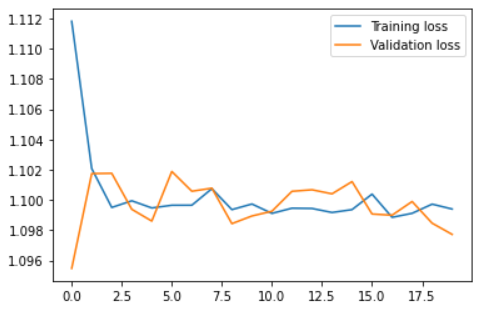
\includegraphics[scale=0.75]{./images/vgg2loss}
	\caption{Training-Validation Loss}
  \end{minipage}
  \hfill
  \begin{minipage}[b]{0.45\textwidth}
    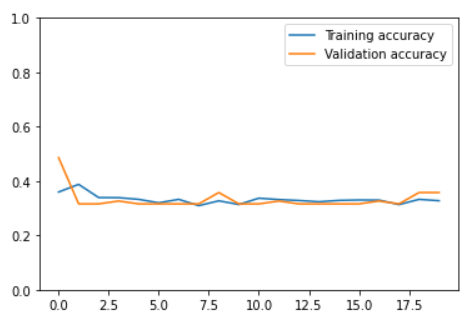
\includegraphics[scale=0.75]{./images/vgg2acc}
	\caption{Training-Validation accuracy}
  \end{minipage}
\end{figure}

\begin{table}[H]
\centering
\begin{tabular}{|c|c|c|c|c|c|c|}
\hline
\rowcolor[rgb]{0.753,0.753,0.753}  \textbf{Modelo}  & \textbf{Loss}                               & \textbf{Accuracy}                           & \begin{tabular}[c]{@{}>{\cellcolor[rgb]{0.753,0.753,0.753}}c@{}}\textbf{Validation}\\\textbf{ Loss} \end{tabular} & \begin{tabular}[c]{@{}>{\cellcolor[rgb]{0.753,0.753,0.753}}c@{}}\textbf{Validation }\\\textbf{ Accuracy} \end{tabular} & \begin{tabular}[c]{@{}>{\cellcolor[rgb]{0.753,0.753,0.753}}c@{}}\textbf{Test }\\\textbf{ Accuracy} \end{tabular} & \begin{tabular}[c]{@{}>{\cellcolor[rgb]{0.753,0.753,0.753}}c@{}}\textbf{Número}\\\textbf{Épocas} \end{tabular}  \\
\hline
\rowcolor[rgb]{0.937,0.937,0.937} DN-V0             &                                             &                                             &                                                                                                                   &                                                                                                                        & \textcolor[rgb]{0.129,0.129,0.129}{0.3264}                                                                       &                                                                                                                 \\
\hline
DN-V1                                               & \textcolor[rgb]{0.129,0.129,0.129}{0.6501}  & \textcolor[rgb]{0.129,0.129,0.129}{0.9588 } & \textcolor[rgb]{0.129,0.129,0.129}{3.1393}                                                                        & \textcolor[rgb]{0.129,0.129,0.129}{0.8333}                                                                             & \textcolor[rgb]{0.129,0.129,0.129}{0.8361}                                                                       & 20                                                                                                              \\
\hline
DN-V2                                               & \textcolor[rgb]{0.129,0.129,0.129}{0.0109 } & \textcolor[rgb]{0.129,0.129,0.129}{0.9973 } & \textcolor[rgb]{0.129,0.129,0.129}{0.1146 }                                                                       & \textcolor[rgb]{0.129,0.129,0.129}{0.9583}                                                                             & \textcolor[rgb]{0.129,0.129,0.129}{0.9597}                                                                       & 20                                                                                                              \\
\hline
DN-V2-reg                                           & \textcolor[rgb]{0.129,0.129,0.129}{0.0883 } & \textcolor[rgb]{0.129,0.129,0.129}{0.9683 } & \textcolor[rgb]{0.129,0.129,0.129}{0.1494 }                                                                       & \textcolor[rgb]{0.129,0.129,0.129}{0.9583}                                                                             & \textcolor[rgb]{0.129,0.129,0.129}{0.9569}                                                                       & 20                                                                                                              \\
\hline
DN-V3                                               & \textcolor[rgb]{0.129,0.129,0.129}{0.0089 } & \textcolor[rgb]{0.129,0.129,0.129}{0.9964 } & \textcolor[rgb]{0.129,0.129,0.129}{0.0924 }                                                                       & \textcolor[rgb]{0.129,0.129,0.129}{0.9826}                                                                             & \textcolor[rgb]{0.129,0.129,0.129}{0.9736}                                                                       & 20                                                                                                              \\
\hline
ResNet-EC                                              & \textcolor[rgb]{0.129,0.129,0.129}{0.2519 } & \textcolor[rgb]{0.129,0.129,0.129}{0.9063 } & \textcolor[rgb]{0.129,0.129,0.129}{0.2134 }                                                                       & \textcolor[rgb]{0.129,0.129,0.129}{0.9236}                                                                             & \textcolor[rgb]{0.129,0.129,0.129}{0.8805}                                                                       & 20                                                                                                              \\
\hline
ResNet-FT                                           & \textcolor[rgb]{0.129,0.129,0.129}{0.0102 } & \textcolor[rgb]{0.129,0.129,0.129}{0.9952 } & \textcolor[rgb]{0.129,0.129,0.129}{0.5594 }                                                                       & \textcolor[rgb]{0.129,0.129,0.129}{0.8576}                                                                             & \textcolor[rgb]{0.129,0.129,0.129}{0.8736}                                                                       & 20                                                                                                              \\
\hline
VGG16-EC                                               & \textcolor[rgb]{0.129,0.129,0.129}{0.1057 } & \textcolor[rgb]{0.129,0.129,0.129}{0.9626 } & \textcolor[rgb]{0.129,0.129,0.129}{0.1063 }                                                                       & \textcolor[rgb]{0.129,0.129,0.129}{0.9618}                                                                             & \textcolor[rgb]{0.129,0.129,0.129}{0.9375}                                                                       & 20                                                                                                              \\
\hline
\rowcolor{green} VGG16-FT                           & \textcolor[rgb]{0.129,0.129,0.129}{1.099}   & \textcolor[rgb]{0.129,0.129,0.129}{0.3159 } & \textcolor[rgb]{0.129,0.129,0.129}{1.0977 }                                                                       & \textcolor[rgb]{0.129,0.129,0.129}{0.3576}                                                                             & \textcolor[rgb]{0.129,0.129,0.129}{0.3388}                                                                       & 20                                                                                                              \\
\hline
\end{tabular}
\caption{Resultados de la ejecución para la red VGG16-TF, mostrando los anteriores}
\end{table}

\begin{table}[htbp]
\begin{center}
\begin{tabular}{l|
>{\columncolor[HTML]{EFEFEF}}l |
>{\columncolor[HTML]{EFEFEF}}l |
>{\columncolor[HTML]{EFEFEF}}l |}
\hline
\multicolumn{1}{|l|}{\cellcolor[HTML]{C0C0C0}\textbf{V-COVID}}  & 0                                        & 235                                       & 0                                       \\ \hline
\multicolumn{1}{|l|}{\cellcolor[HTML]{C0C0C0}\textbf{V-Normal}} & 0                                        & 244                                       & 0                                       \\ \hline
\multicolumn{1}{|l|}{\cellcolor[HTML]{C0C0C0}\textbf{V-Neum.}}  & 0                                        & 241                                       & 0                                       \\ \hline
                                                                & \cellcolor[HTML]{C0C0C0}\textbf{P-COVID} & \cellcolor[HTML]{C0C0C0}\textbf{P-Normal} & \cellcolor[HTML]{C0C0C0}\textbf{P-Neum} \\ \cline{2-4}
\end{tabular}
\end{center}
\caption{Matriz de confusión para la red VGG16-TF}
\end{table}

Los resultados son realmente malos, no se aprecia ningún tipo de aprendizaje, ya que son muy cercanos a los que obtuvimos con DN-V0, donde no había ningún tipo de entrenamiento. De hecho, si vemos la matriz de confusión, el modelo siempre predice que todas las imágenes pertenecen a la clase NORMAL.\\

La ejecución se ha hecho en las mismas condiciones que los demás modelos, luego solo podemos concluir que este modelo no funciona para nada bien en su versión fine tunning.

\subsection{InceptionV3}

\subsubsection{InceptionV3-EC}

\begin{figure}[H]
  \centering
  \begin{minipage}[b]{0.45\textwidth}
    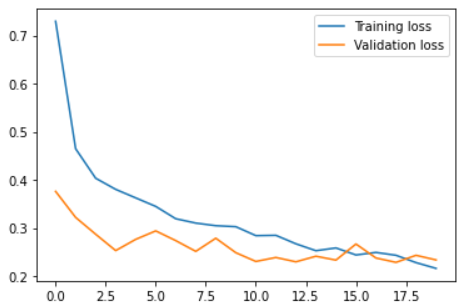
\includegraphics[scale=0.75]{./images/inception1loss}
	\caption{Training-Validation Loss}
  \end{minipage}
  \hfill
  \begin{minipage}[b]{0.45\textwidth}
    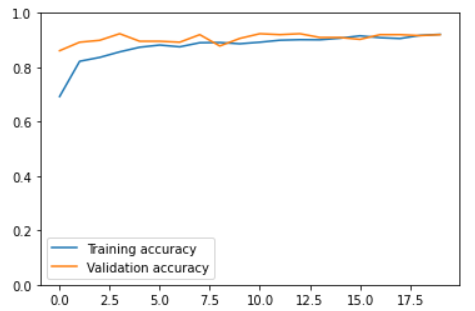
\includegraphics[scale=0.75]{./images/inception1acc}
	\caption{Training-Validation accuracy}
  \end{minipage}
\end{figure}

\begin{table}[H]
\centering
\begin{tabular}{|c|c|c|c|c|c|c|}
\hline
\rowcolor[rgb]{0.753,0.753,0.753}  \textbf{Modelo}  & \textbf{Loss}                               & \textbf{Accuracy}                           & \begin{tabular}[c]{@{}>{\cellcolor[rgb]{0.753,0.753,0.753}}c@{}}\textbf{Validation}\\\textbf{ Loss} \end{tabular} & \begin{tabular}[c]{@{}>{\cellcolor[rgb]{0.753,0.753,0.753}}c@{}}\textbf{Validation }\\\textbf{ Accuracy} \end{tabular} & \begin{tabular}[c]{@{}>{\cellcolor[rgb]{0.753,0.753,0.753}}c@{}}\textbf{Test }\\\textbf{ Accuracy} \end{tabular} & \begin{tabular}[c]{@{}>{\cellcolor[rgb]{0.753,0.753,0.753}}c@{}}\textbf{Número}\\\textbf{Épocas} \end{tabular}  \\
\hline
\rowcolor[rgb]{0.937,0.937,0.937} DN-V0             &                                             &                                             &                                                                                                                   &                                                                                                                        & \textcolor[rgb]{0.129,0.129,0.129}{0.3264}                                                                       &                                                                                                                 \\
\hline
DN-V1                                               & \textcolor[rgb]{0.129,0.129,0.129}{0.6501}  & \textcolor[rgb]{0.129,0.129,0.129}{0.9588 } & \textcolor[rgb]{0.129,0.129,0.129}{3.1393}                                                                        & \textcolor[rgb]{0.129,0.129,0.129}{0.8333}                                                                             & \textcolor[rgb]{0.129,0.129,0.129}{0.8361}                                                                       & 20                                                                                                              \\
\hline
DN-V2                                               & \textcolor[rgb]{0.129,0.129,0.129}{0.0109 } & \textcolor[rgb]{0.129,0.129,0.129}{0.9973 } & \textcolor[rgb]{0.129,0.129,0.129}{0.1146 }                                                                       & \textcolor[rgb]{0.129,0.129,0.129}{0.9583}                                                                             & \textcolor[rgb]{0.129,0.129,0.129}{0.9597}                                                                       & 20                                                                                                              \\
\hline
DN-V2-reg                                           & \textcolor[rgb]{0.129,0.129,0.129}{0.0883 } & \textcolor[rgb]{0.129,0.129,0.129}{0.9683 } & \textcolor[rgb]{0.129,0.129,0.129}{0.1494 }                                                                       & \textcolor[rgb]{0.129,0.129,0.129}{0.9583}                                                                             & \textcolor[rgb]{0.129,0.129,0.129}{0.9569}                                                                       & 20                                                                                                              \\
\hline
DN-V3                                               & \textcolor[rgb]{0.129,0.129,0.129}{0.0089 } & \textcolor[rgb]{0.129,0.129,0.129}{0.9964 } & \textcolor[rgb]{0.129,0.129,0.129}{0.0924 }                                                                       & \textcolor[rgb]{0.129,0.129,0.129}{0.9826}                                                                             & \textcolor[rgb]{0.129,0.129,0.129}{0.9736}                                                                       & 20                                                                                                              \\
\hline
ResNet-EC                                              & \textcolor[rgb]{0.129,0.129,0.129}{0.2519 } & \textcolor[rgb]{0.129,0.129,0.129}{0.9063 } & \textcolor[rgb]{0.129,0.129,0.129}{0.2134 }                                                                       & \textcolor[rgb]{0.129,0.129,0.129}{0.9236}                                                                             & \textcolor[rgb]{0.129,0.129,0.129}{0.8805}                                                                       & 20                                                                                                              \\
\hline
ResNet-FT                                           & \textcolor[rgb]{0.129,0.129,0.129}{0.0102 } & \textcolor[rgb]{0.129,0.129,0.129}{0.9952 } & \textcolor[rgb]{0.129,0.129,0.129}{0.5594 }                                                                       & \textcolor[rgb]{0.129,0.129,0.129}{0.8576}                                                                             & \textcolor[rgb]{0.129,0.129,0.129}{0.8736}                                                                       & 20                                                                                                              \\
\hline
VGG16-EC                                               & \textcolor[rgb]{0.129,0.129,0.129}{0.1057 } & \textcolor[rgb]{0.129,0.129,0.129}{0.9626 } & \textcolor[rgb]{0.129,0.129,0.129}{0.1063 }                                                                       & \textcolor[rgb]{0.129,0.129,0.129}{0.9618}                                                                             & \textcolor[rgb]{0.129,0.129,0.129}{0.9375}                                                                       & 20                                                                                                              \\
\hline
VGG16-FT                                            & \textcolor[rgb]{0.129,0.129,0.129}{1.099}   & \textcolor[rgb]{0.129,0.129,0.129}{0.3159 } & \textcolor[rgb]{0.129,0.129,0.129}{1.0977 }                                                                       & \textcolor[rgb]{0.129,0.129,0.129}{0.3576}                                                                             & \textcolor[rgb]{0.129,0.129,0.129}{0.3388}                                                                       & 20                                                                                                              \\
\hline
\rowcolor{green} InceptionV3-EC                        & \textcolor[rgb]{0.129,0.129,0.129}{0.2194 } & \textcolor[rgb]{0.129,0.129,0.129}{0.9231 } & \textcolor[rgb]{0.129,0.129,0.129}{0.2337 }                                                                       & \textcolor[rgb]{0.129,0.129,0.129}{0.9201}                                                                             & \textcolor[rgb]{0.129,0.129,0.129}{0.8903}                                                                       & 20                                                                                                              \\
\hline
\end{tabular}

\caption{Resultados de la ejecución para la red InceptionV3-EC, mostrando los anteriores}
\end{table}

\begin{table}[htbp]
\begin{center}
\begin{tabular}{l|
>{\columncolor[HTML]{EFEFEF}}l |
>{\columncolor[HTML]{EFEFEF}}l |
>{\columncolor[HTML]{EFEFEF}}l |}
\hline
\multicolumn{1}{|l|}{\cellcolor[HTML]{C0C0C0}\textbf{V-COVID}}  & 224                                      & 4                                         & 7                                       \\ \hline
\multicolumn{1}{|l|}{\cellcolor[HTML]{C0C0C0}\textbf{V-Normal}} & 17                                       & 210                                       & 17                                      \\ \hline
\multicolumn{1}{|l|}{\cellcolor[HTML]{C0C0C0}\textbf{V-Neum.}}  & 11                                       & 23                                        & 207                                     \\ \hline
                                                                & \cellcolor[HTML]{C0C0C0}\textbf{P-COVID} & \cellcolor[HTML]{C0C0C0}\textbf{P-Normal} & \cellcolor[HTML]{C0C0C0}\textbf{P-Neum} \\ \cline{2-4}
\end{tabular}
\end{center}
\caption{Matriz de confusión para la red InceptionV3-EC}
\end{table}


En general es un buen resultado, aunque no es excepcional comparándolo algunos de sus con sus homólogos anteriores.\\

\subsubsection{InceptionV3-FT}

\begin{figure}[H]
  \centering
  \begin{minipage}[b]{0.45\textwidth}
    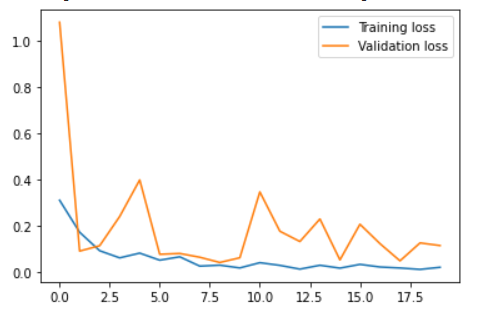
\includegraphics[scale=0.75]{./images/inception2loss}
	\caption{Training-Validation Loss}
  \end{minipage}
  \hfill
  \begin{minipage}[b]{0.45\textwidth}
    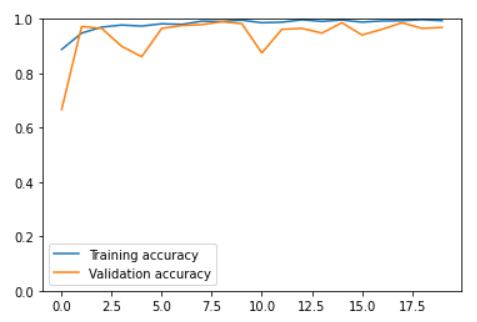
\includegraphics[scale=0.75]{./images/inception2acc}
	\caption{Training-Validation accuracy}
  \end{minipage}
\end{figure}

\begin{table}[H]
\centering
\begin{tabular}{|c|c|c|c|c|c|c|}
\hline
\rowcolor[rgb]{0.753,0.753,0.753}  \textbf{Modelo}  & \textbf{Loss}                               & \textbf{Accuracy}                           & \begin{tabular}[c]{@{}>{\cellcolor[rgb]{0.753,0.753,0.753}}c@{}}\textbf{Validation}\\\textbf{ Loss} \end{tabular} & \begin{tabular}[c]{@{}>{\cellcolor[rgb]{0.753,0.753,0.753}}c@{}}\textbf{Validation }\\\textbf{ Accuracy} \end{tabular} & \begin{tabular}[c]{@{}>{\cellcolor[rgb]{0.753,0.753,0.753}}c@{}}\textbf{Test }\\\textbf{ Accuracy} \end{tabular} & \begin{tabular}[c]{@{}>{\cellcolor[rgb]{0.753,0.753,0.753}}c@{}}\textbf{Número}\\\textbf{Épocas} \end{tabular}  \\
\hline
\rowcolor[rgb]{0.937,0.937,0.937} DN-V0             &                                             &                                             &                                                                                                                   &                                                                                                                        & \textcolor[rgb]{0.129,0.129,0.129}{0.3264}                                                                       &                                                                                                                 \\
\hline
DN-V1                                               & \textcolor[rgb]{0.129,0.129,0.129}{0.6501}  & \textcolor[rgb]{0.129,0.129,0.129}{0.9588 } & \textcolor[rgb]{0.129,0.129,0.129}{3.1393}                                                                        & \textcolor[rgb]{0.129,0.129,0.129}{0.8333}                                                                             & \textcolor[rgb]{0.129,0.129,0.129}{0.8361}                                                                       & 20                                                                                                              \\
\hline
DN-V2                                               & \textcolor[rgb]{0.129,0.129,0.129}{0.0109 } & \textcolor[rgb]{0.129,0.129,0.129}{0.9973 } & \textcolor[rgb]{0.129,0.129,0.129}{0.1146 }                                                                       & \textcolor[rgb]{0.129,0.129,0.129}{0.9583}                                                                             & \textcolor[rgb]{0.129,0.129,0.129}{0.9597}                                                                       & 20                                                                                                              \\
\hline
DN-V2-reg                                           & \textcolor[rgb]{0.129,0.129,0.129}{0.0883 } & \textcolor[rgb]{0.129,0.129,0.129}{0.9683 } & \textcolor[rgb]{0.129,0.129,0.129}{0.1494 }                                                                       & \textcolor[rgb]{0.129,0.129,0.129}{0.9583}                                                                             & \textcolor[rgb]{0.129,0.129,0.129}{0.9569}                                                                       & 20                                                                                                              \\
\hline
DN-V3                                               & \textcolor[rgb]{0.129,0.129,0.129}{0.0089 } & \textcolor[rgb]{0.129,0.129,0.129}{0.9964 } & \textcolor[rgb]{0.129,0.129,0.129}{0.0924 }                                                                       & \textcolor[rgb]{0.129,0.129,0.129}{0.9826}                                                                             & \textcolor[rgb]{0.129,0.129,0.129}{0.9736}                                                                       & 20                                                                                                              \\
\hline
ResNet-EC                                              & \textcolor[rgb]{0.129,0.129,0.129}{0.2519 } & \textcolor[rgb]{0.129,0.129,0.129}{0.9063 } & \textcolor[rgb]{0.129,0.129,0.129}{0.2134 }                                                                       & \textcolor[rgb]{0.129,0.129,0.129}{0.9236}                                                                             & \textcolor[rgb]{0.129,0.129,0.129}{0.8805}                                                                       & 20                                                                                                              \\
\hline
ResNet-FT                                           & \textcolor[rgb]{0.129,0.129,0.129}{0.0102 } & \textcolor[rgb]{0.129,0.129,0.129}{0.9952 } & \textcolor[rgb]{0.129,0.129,0.129}{0.5594 }                                                                       & \textcolor[rgb]{0.129,0.129,0.129}{0.8576}                                                                             & \textcolor[rgb]{0.129,0.129,0.129}{0.8736}                                                                       & 20                                                                                                              \\
\hline
VGG16-EC                                               & \textcolor[rgb]{0.129,0.129,0.129}{0.1057 } & \textcolor[rgb]{0.129,0.129,0.129}{0.9626 } & \textcolor[rgb]{0.129,0.129,0.129}{0.1063 }                                                                       & \textcolor[rgb]{0.129,0.129,0.129}{0.9618}                                                                             & \textcolor[rgb]{0.129,0.129,0.129}{0.9375}                                                                       & 20                                                                                                              \\
\hline
VGG16-FT                                            & \textcolor[rgb]{0.129,0.129,0.129}{1.099}   & \textcolor[rgb]{0.129,0.129,0.129}{0.3159 } & \textcolor[rgb]{0.129,0.129,0.129}{1.0977 }                                                                       & \textcolor[rgb]{0.129,0.129,0.129}{0.3576}                                                                             & \textcolor[rgb]{0.129,0.129,0.129}{0.3388}                                                                       & 20                                                                                                              \\
\hline
InceptionV3-EC                                         & \textcolor[rgb]{0.129,0.129,0.129}{0.2194 } & \textcolor[rgb]{0.129,0.129,0.129}{0.9231 } & \textcolor[rgb]{0.129,0.129,0.129}{0.2337 }                                                                       & \textcolor[rgb]{0.129,0.129,0.129}{0.9201}                                                                             & \textcolor[rgb]{0.129,0.129,0.129}{0.8903}                                                                       & 20                                                                                                              \\
\hline
\rowcolor{green} InceptionV3-FT                                      & \textcolor[rgb]{0.129,0.129,0.129}{0.0146 } & \textcolor[rgb]{0.129,0.129,0.129}{0.9953 } & \textcolor[rgb]{0.129,0.129,0.129}{0.1142 }                                                                       & \textcolor[rgb]{0.129,0.129,0.129}{0.9688}                                                                             & \textcolor[rgb]{0.129,0.129,0.129}{0.9792}                                                                       & 20                                                                                                              \\
\hline

\end{tabular}
\caption{Resultados de la ejecución para la red InceptionV3-FT, mostrando los anteriores}
\end{table}

\begin{table}[htbp]
\begin{center}
\begin{tabular}{l|
>{\columncolor[HTML]{EFEFEF}}l |
>{\columncolor[HTML]{EFEFEF}}l |
>{\columncolor[HTML]{EFEFEF}}l |}
\hline
\multicolumn{1}{|l|}{\cellcolor[HTML]{C0C0C0}\textbf{V-COVID}}  & 233                                      & 1                                         & 1                                       \\ \hline
\multicolumn{1}{|l|}{\cellcolor[HTML]{C0C0C0}\textbf{V-Normal}} & 0                                        & 243                                       & 1                                       \\ \hline
\multicolumn{1}{|l|}{\cellcolor[HTML]{C0C0C0}\textbf{V-Neum.}}  & 1                                        & 11                                        & 229                                     \\ \hline
                                                                & \cellcolor[HTML]{C0C0C0}\textbf{P-COVID} & \cellcolor[HTML]{C0C0C0}\textbf{P-Normal} & \cellcolor[HTML]{C0C0C0}\textbf{P-Neum} \\ \cline{2-4}
\end{tabular}
\end{center}
\caption{Matriz de confusión para la red InceptionV3-FT}
\end{table}

Ahora sí que hemos dado un salto de calidad respecto al anterior, que está a la altura del mejor modelo hasta el momento (DN-V3). La única dificultad que encuentra el modelo está a la hora de clasificar imágenes de la clase de otros tipos de Neumonías Víricas, confundiéndolas con imágenes de pulmones sanos.

\subsection{Xception}

\subsubsection{Xception-EC}

\begin{figure}[H]
  \centering
  \begin{minipage}[b]{0.45\textwidth}
    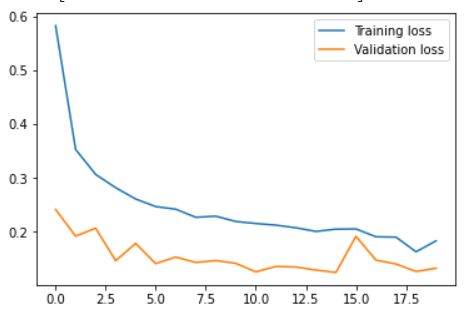
\includegraphics[scale=0.75]{./images/xception1loss}
	\caption{Training-Validation Loss}
  \end{minipage}
  \hfill
  \begin{minipage}[b]{0.45\textwidth}
    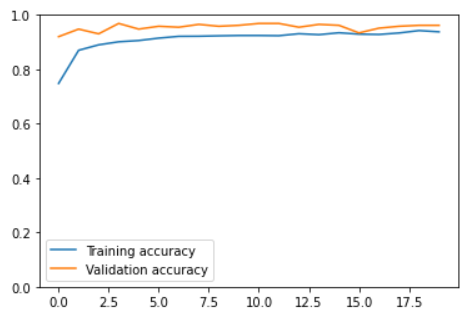
\includegraphics[scale=0.75]{./images/xception1acc}
	\caption{Training-Validation accuracy}
  \end{minipage}
\end{figure}

\begin{table}[H]
\centering
\begin{tabular}{|c|c|c|c|c|c|c|}
\hline
\rowcolor[rgb]{0.753,0.753,0.753}  \textbf{Modelo}  & \textbf{Loss}                               & \textbf{Accuracy}                           & \begin{tabular}[c]{@{}>{\cellcolor[rgb]{0.753,0.753,0.753}}c@{}}\textbf{Validation}\\\textbf{ Loss} \end{tabular} & \begin{tabular}[c]{@{}>{\cellcolor[rgb]{0.753,0.753,0.753}}c@{}}\textbf{Validation }\\\textbf{ Accuracy} \end{tabular} & \begin{tabular}[c]{@{}>{\cellcolor[rgb]{0.753,0.753,0.753}}c@{}}\textbf{Test }\\\textbf{ Accuracy} \end{tabular} & \begin{tabular}[c]{@{}>{\cellcolor[rgb]{0.753,0.753,0.753}}c@{}}\textbf{Número}\\\textbf{Épocas} \end{tabular}  \\
\hline
\rowcolor[rgb]{0.937,0.937,0.937} DN-V0             &                                             &                                             &                                                                                                                   &                                                                                                                        & \textcolor[rgb]{0.129,0.129,0.129}{0.3264}                                                                       &                                                                                                                 \\
\hline
DN-V1                                               & \textcolor[rgb]{0.129,0.129,0.129}{0.6501}  & \textcolor[rgb]{0.129,0.129,0.129}{0.9588 } & \textcolor[rgb]{0.129,0.129,0.129}{3.1393}                                                                        & \textcolor[rgb]{0.129,0.129,0.129}{0.8333}                                                                             & \textcolor[rgb]{0.129,0.129,0.129}{0.8361}                                                                       & 20                                                                                                              \\
\hline
DN-V2                                               & \textcolor[rgb]{0.129,0.129,0.129}{0.0109 } & \textcolor[rgb]{0.129,0.129,0.129}{0.9973 } & \textcolor[rgb]{0.129,0.129,0.129}{0.1146 }                                                                       & \textcolor[rgb]{0.129,0.129,0.129}{0.9583}                                                                             & \textcolor[rgb]{0.129,0.129,0.129}{0.9597}                                                                       & 20                                                                                                              \\
\hline
DN-V2-reg                                           & \textcolor[rgb]{0.129,0.129,0.129}{0.0883 } & \textcolor[rgb]{0.129,0.129,0.129}{0.9683 } & \textcolor[rgb]{0.129,0.129,0.129}{0.1494 }                                                                       & \textcolor[rgb]{0.129,0.129,0.129}{0.9583}                                                                             & \textcolor[rgb]{0.129,0.129,0.129}{0.9569}                                                                       & 20                                                                                                              \\
\hline
DN-V3                                               & \textcolor[rgb]{0.129,0.129,0.129}{0.0089 } & \textcolor[rgb]{0.129,0.129,0.129}{0.9964 } & \textcolor[rgb]{0.129,0.129,0.129}{0.0924 }                                                                       & \textcolor[rgb]{0.129,0.129,0.129}{0.9826}                                                                             & \textcolor[rgb]{0.129,0.129,0.129}{0.9736}                                                                       & 20                                                                                                              \\
\hline
ResNet-EC                                              & \textcolor[rgb]{0.129,0.129,0.129}{0.2519 } & \textcolor[rgb]{0.129,0.129,0.129}{0.9063 } & \textcolor[rgb]{0.129,0.129,0.129}{0.2134 }                                                                       & \textcolor[rgb]{0.129,0.129,0.129}{0.9236}                                                                             & \textcolor[rgb]{0.129,0.129,0.129}{0.8805}                                                                       & 20                                                                                                              \\
\hline
ResNet-FT                                           & \textcolor[rgb]{0.129,0.129,0.129}{0.0102 } & \textcolor[rgb]{0.129,0.129,0.129}{0.9952 } & \textcolor[rgb]{0.129,0.129,0.129}{0.5594 }                                                                       & \textcolor[rgb]{0.129,0.129,0.129}{0.8576}                                                                             & \textcolor[rgb]{0.129,0.129,0.129}{0.8736}                                                                       & 20                                                                                                              \\
\hline
VGG16-EC                                               & \textcolor[rgb]{0.129,0.129,0.129}{0.1057 } & \textcolor[rgb]{0.129,0.129,0.129}{0.9626 } & \textcolor[rgb]{0.129,0.129,0.129}{0.1063 }                                                                       & \textcolor[rgb]{0.129,0.129,0.129}{0.9618}                                                                             & \textcolor[rgb]{0.129,0.129,0.129}{0.9375}                                                                       & 20                                                                                                              \\
\hline
VGG16-FT                                            & \textcolor[rgb]{0.129,0.129,0.129}{1.099}   & \textcolor[rgb]{0.129,0.129,0.129}{0.3159 } & \textcolor[rgb]{0.129,0.129,0.129}{1.0977 }                                                                       & \textcolor[rgb]{0.129,0.129,0.129}{0.3576}                                                                             & \textcolor[rgb]{0.129,0.129,0.129}{0.3388}                                                                       & 20                                                                                                              \\
\hline
InceptionV3-EC                                         & \textcolor[rgb]{0.129,0.129,0.129}{0.2194 } & \textcolor[rgb]{0.129,0.129,0.129}{0.9231 } & \textcolor[rgb]{0.129,0.129,0.129}{0.2337 }                                                                       & \textcolor[rgb]{0.129,0.129,0.129}{0.9201}                                                                             & \textcolor[rgb]{0.129,0.129,0.129}{0.8903}                                                                       & 20                                                                                                              \\
\hline
InceptionV3-FT                                      & \textcolor[rgb]{0.129,0.129,0.129}{0.0146 } & \textcolor[rgb]{0.129,0.129,0.129}{0.9953 } & \textcolor[rgb]{0.129,0.129,0.129}{0.1142 }                                                                       & \textcolor[rgb]{0.129,0.129,0.129}{0.9688}                                                                             & \textcolor[rgb]{0.129,0.129,0.129}{0.9792}                                                                       & 20                                                                                                              \\
\hline
\rowcolor{green} Xception-EC                           & \textcolor[rgb]{0.129,0.129,0.129}{0.1746 } & \textcolor[rgb]{0.129,0.129,0.129}{0.9405 } & \textcolor[rgb]{0.129,0.129,0.129}{0.1319 }                                                                       & \textcolor[rgb]{0.129,0.129,0.129}{0.9618}                                                                             & \textcolor[rgb]{0.129,0.129,0.129}{0.9153}                                                                       & 20                                                                                                              \\
\hline
\end{tabular}
\caption{Resultados de la ejecución para la red Xception-EC, mostrando los anteriores}
\end{table}

\begin{table}[htbp]
\begin{center}
\begin{tabular}{l|
>{\columncolor[HTML]{EFEFEF}}l |
>{\columncolor[HTML]{EFEFEF}}l |
>{\columncolor[HTML]{EFEFEF}}l |}
\hline
\multicolumn{1}{|l|}{\cellcolor[HTML]{C0C0C0}\textbf{V-COVID}}  & 231                                      & 2                                         & 2                                       \\ \hline
\multicolumn{1}{|l|}{\cellcolor[HTML]{C0C0C0}\textbf{V-Normal}} & 2                                        & 223                                       & 19                                      \\ \hline
\multicolumn{1}{|l|}{\cellcolor[HTML]{C0C0C0}\textbf{V-Neum.}}  & 8                                        & 28                                        & 205                                     \\ \hline
                                                                & \cellcolor[HTML]{C0C0C0}\textbf{P-COVID} & \cellcolor[HTML]{C0C0C0}\textbf{P-Normal} & \cellcolor[HTML]{C0C0C0}\textbf{P-Neum} \\ \cline{2-4}
\end{tabular}
\end{center}
\caption{Matriz de confusión para la red Xception-EC}
\end{table}

Buenos resultados, que recuerdan bastante a la versión de InceptionV3-EC, que tiene sentido al ser modelo similares.\\

\subsubsection{Xception-FT}

\begin{figure}[H]
  \centering
  \begin{minipage}[b]{0.45\textwidth}
    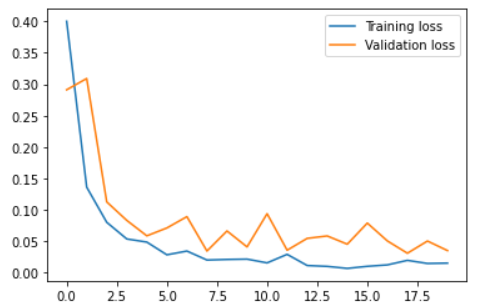
\includegraphics[scale=0.75]{./images/xception2aloss}
	\caption{Training-Validation Loss}
  \end{minipage}
  \hfill
  \begin{minipage}[b]{0.45\textwidth}
    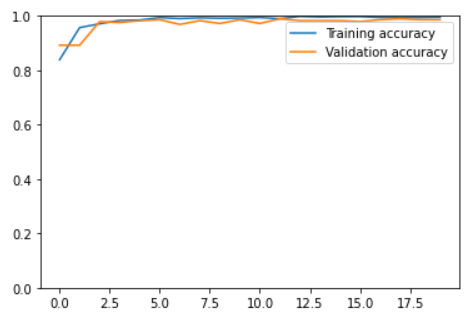
\includegraphics[scale=0.75]{./images/xception2acc}
	\caption{Training-Validation accuracy}
  \end{minipage}
\end{figure}

\begin{table}[H]
\centering
\begin{tabular}{|c|c|c|c|c|c|c|}
\hline
\rowcolor[rgb]{0.753,0.753,0.753}  \textbf{Modelo}  & \textbf{Loss}                               & \textbf{Accuracy}                           & \begin{tabular}[c]{@{}>{\cellcolor[rgb]{0.753,0.753,0.753}}c@{}}\textbf{Validation}\\\textbf{ Loss} \end{tabular} & \begin{tabular}[c]{@{}>{\cellcolor[rgb]{0.753,0.753,0.753}}c@{}}\textbf{Validation }\\\textbf{ Accuracy} \end{tabular} & \begin{tabular}[c]{@{}>{\cellcolor[rgb]{0.753,0.753,0.753}}c@{}}\textbf{Test }\\\textbf{ Accuracy} \end{tabular} & \begin{tabular}[c]{@{}>{\cellcolor[rgb]{0.753,0.753,0.753}}c@{}}\textbf{Número}\\\textbf{Épocas} \end{tabular}  \\
\hline
\rowcolor[rgb]{0.937,0.937,0.937} DN-V0             &                                             &                                             &                                                                                                                   &                                                                                                                        & \textcolor[rgb]{0.129,0.129,0.129}{0.3264}                                                                       &                                                                                                                 \\
\hline
DN-V1                                               & \textcolor[rgb]{0.129,0.129,0.129}{0.6501}  & \textcolor[rgb]{0.129,0.129,0.129}{0.9588 } & \textcolor[rgb]{0.129,0.129,0.129}{3.1393}                                                                        & \textcolor[rgb]{0.129,0.129,0.129}{0.8333}                                                                             & \textcolor[rgb]{0.129,0.129,0.129}{0.8361}                                                                       & 20                                                                                                              \\
\hline
DN-V2                                               & \textcolor[rgb]{0.129,0.129,0.129}{0.0109 } & \textcolor[rgb]{0.129,0.129,0.129}{0.9973 } & \textcolor[rgb]{0.129,0.129,0.129}{0.1146 }                                                                       & \textcolor[rgb]{0.129,0.129,0.129}{0.9583}                                                                             & \textcolor[rgb]{0.129,0.129,0.129}{0.9597}                                                                       & 20                                                                                                              \\
\hline
DN-V2-reg                                           & \textcolor[rgb]{0.129,0.129,0.129}{0.0883 } & \textcolor[rgb]{0.129,0.129,0.129}{0.9683 } & \textcolor[rgb]{0.129,0.129,0.129}{0.1494 }                                                                       & \textcolor[rgb]{0.129,0.129,0.129}{0.9583}                                                                             & \textcolor[rgb]{0.129,0.129,0.129}{0.9569}                                                                       & 20                                                                                                              \\
\hline
DN-V3                                               & \textcolor[rgb]{0.129,0.129,0.129}{0.0089 } & \textcolor[rgb]{0.129,0.129,0.129}{0.9964 } & \textcolor[rgb]{0.129,0.129,0.129}{0.0924 }                                                                       & \textcolor[rgb]{0.129,0.129,0.129}{0.9826}                                                                             & \textcolor[rgb]{0.129,0.129,0.129}{0.9736}                                                                       & 20                                                                                                              \\
\hline
ResNet-EC                                              & \textcolor[rgb]{0.129,0.129,0.129}{0.2519 } & \textcolor[rgb]{0.129,0.129,0.129}{0.9063 } & \textcolor[rgb]{0.129,0.129,0.129}{0.2134 }                                                                       & \textcolor[rgb]{0.129,0.129,0.129}{0.9236}                                                                             & \textcolor[rgb]{0.129,0.129,0.129}{0.8805}                                                                       & 20                                                                                                              \\
\hline
ResNet-FT                                           & \textcolor[rgb]{0.129,0.129,0.129}{0.0102 } & \textcolor[rgb]{0.129,0.129,0.129}{0.9952 } & \textcolor[rgb]{0.129,0.129,0.129}{0.5594 }                                                                       & \textcolor[rgb]{0.129,0.129,0.129}{0.8576}                                                                             & \textcolor[rgb]{0.129,0.129,0.129}{0.8736}                                                                       & 20                                                                                                              \\
\hline
VGG16-EC                                               & \textcolor[rgb]{0.129,0.129,0.129}{0.1057 } & \textcolor[rgb]{0.129,0.129,0.129}{0.9626 } & \textcolor[rgb]{0.129,0.129,0.129}{0.1063 }                                                                       & \textcolor[rgb]{0.129,0.129,0.129}{0.9618}                                                                             & \textcolor[rgb]{0.129,0.129,0.129}{0.9375}                                                                       & 20                                                                                                              \\
\hline
VGG16-FT                                            & \textcolor[rgb]{0.129,0.129,0.129}{1.099}   & \textcolor[rgb]{0.129,0.129,0.129}{0.3159 } & \textcolor[rgb]{0.129,0.129,0.129}{1.0977 }                                                                       & \textcolor[rgb]{0.129,0.129,0.129}{0.3576}                                                                             & \textcolor[rgb]{0.129,0.129,0.129}{0.3388}                                                                       & 20                                                                                                              \\
\hline
InceptionV3-EC                                         & \textcolor[rgb]{0.129,0.129,0.129}{0.2194 } & \textcolor[rgb]{0.129,0.129,0.129}{0.9231 } & \textcolor[rgb]{0.129,0.129,0.129}{0.2337 }                                                                       & \textcolor[rgb]{0.129,0.129,0.129}{0.9201}                                                                             & \textcolor[rgb]{0.129,0.129,0.129}{0.8903}                                                                       & 20                                                                                                              \\
\hline
InceptionV3-FT                                      & \textcolor[rgb]{0.129,0.129,0.129}{0.0146 } & \textcolor[rgb]{0.129,0.129,0.129}{0.9953 } & \textcolor[rgb]{0.129,0.129,0.129}{0.1142 }                                                                       & \textcolor[rgb]{0.129,0.129,0.129}{0.9688}                                                                             & \textcolor[rgb]{0.129,0.129,0.129}{0.9792}                                                                       & 20                                                                                                              \\
\hline
Xception-EC                                            & \textcolor[rgb]{0.129,0.129,0.129}{0.1746 } & \textcolor[rgb]{0.129,0.129,0.129}{0.9405 } & \textcolor[rgb]{0.129,0.129,0.129}{0.1319 }                                                                       & \textcolor[rgb]{0.129,0.129,0.129}{0.9618}                                                                             & \textcolor[rgb]{0.129,0.129,0.129}{0.9153}                                                                       & 20                                                                                                              \\
\hline
\rowcolor{green} Xception-FT                        & \textcolor[rgb]{0.129,0.129,0.129}{0.0157 } & \textcolor[rgb]{0.129,0.129,0.129}{0.9946 } & \textcolor[rgb]{0.129,0.129,0.129}{0.0352 }                                                                       & \textcolor[rgb]{0.129,0.129,0.129}{0.9861}                                                                             & \textcolor[rgb]{0.129,0.129,0.129}{0.9875}                                                                       & 20                                                                                                              \\
\hline
\end{tabular}
\caption{Resultados de la ejecución para la red Xception-FT mostrando los anteriores}
\end{table}


\begin{table}[htbp]
\begin{center}
\begin{tabular}{l|
>{\columncolor[HTML]{EFEFEF}}l |
>{\columncolor[HTML]{EFEFEF}}l |
>{\columncolor[HTML]{EFEFEF}}l |}
\hline
\multicolumn{1}{|l|}{\cellcolor[HTML]{C0C0C0}\textbf{V-COVID}}  & 234                                      & 0                                         & 1                                       \\ \hline
\multicolumn{1}{|l|}{\cellcolor[HTML]{C0C0C0}\textbf{V-Normal}} & 0                                        & 244                                       & 0                                       \\ \hline
\multicolumn{1}{|l|}{\cellcolor[HTML]{C0C0C0}\textbf{V-Neum.}}  & 0                                        & 8                                         & 233                                     \\ \hline
                                                                & \cellcolor[HTML]{C0C0C0}\textbf{P-COVID} & \cellcolor[HTML]{C0C0C0}\textbf{P-Normal} & \cellcolor[HTML]{C0C0C0}\textbf{P-Neum} \\ \cline{2-4}
\end{tabular}
\end{center}
\caption{Matriz de confusión para la red Xception-FT}
\end{table}

Estos resultados son los mejores obtenidos hasta el momento, con casi un 99\% de precisión en el conjunto test. De hecho, podemos ver que solo ha fallado en la clasificación de 9 imágenes de las 720 que conforman el conjunto test.\\

Observando la matriz de confusión vemos que, al igual que InceptionV3-FT,  8 de los 9 errores han sido por predecir la clase Normal cuando era Neumonía Vírica. Esto contrasta con el que ha sido nuestro segundo mejor modelo, el de DenseNet con fine tunning, que predecía Neumonía Vírica cuando era Normal.

\subsection{Entrenamiento de una red desde 0}

\subsubsection{Primera Versión: Red más compleja}
Hemos decidido también hacer una prueba entrenando una red desde 0(``from scratch"), para ver cómo se adaptaba al conjunto de entrenamiento en caso de no usar pesos preestablecidos del challenge de Imagenet, con lo que la única información de la que dispondrá la deberá extraer de nuestro conjunto de entrenamiento. \\

La red que decidimos usar fue una red que desarrolló David para el bonus de la práctica 2, adaptándola para este problema. Se trata de una red elaborada, la cual posee módulos residuales donde se calcula información a múltiples escalas. Además,  tiene un enfoque denso donde parte de la información de capas superiores se comunica a capas más avanzadas de la red.  Puesto que hicimos pruebas que no salieron bien probablemente por la dimensión de la red y el número de parámetros que tenía frente al tamaño del conjunto de entrenamiento, decidimos simplificarla un poco disminuyendo el número de módulos residuales y otros cambios. El esquema de la red es el siguiente:

\begin{figure}[H]
  \centering
    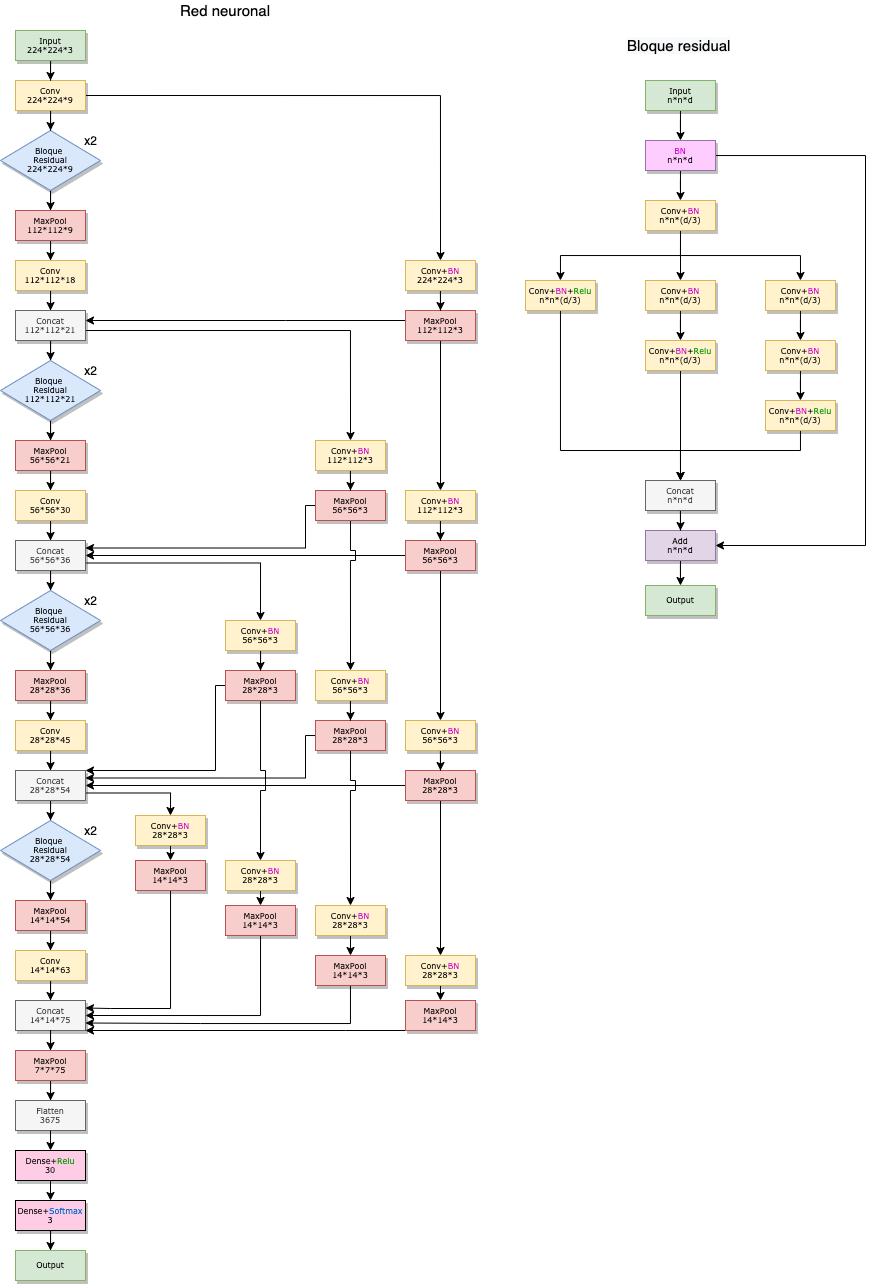
\includegraphics[scale=0.5]{./images/ScratchDavid.png}
	\caption{Descripción de la red neuronal a entrenar desde 0 basada en la red de David}

\end{figure}


\begin{figure}[H]
  \centering
  \begin{minipage}[b]{0.45\textwidth}
    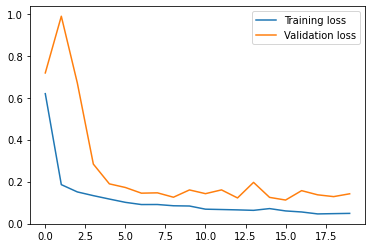
\includegraphics[scale=0.75]{./images/davidloss}
	\caption{Training-Validation Loss}
  \end{minipage}
  \hfill
  \begin{minipage}[b]{0.45\textwidth}
    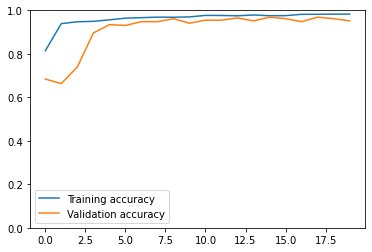
\includegraphics[scale=0.75]{./images/davidacc}
	\caption{Training-Validation accuracy}
  \end{minipage}
\end{figure}


\begin{table}[H]
\centering
\begin{tabular}{|c|c|c|c|c|c|c|}
\hline
\rowcolor[rgb]{0.753,0.753,0.753}  \textbf{Modelo}  & \textbf{Loss}                               & \textbf{Accuracy}                           & \begin{tabular}[c]{@{}>{\cellcolor[rgb]{0.753,0.753,0.753}}c@{}}\textbf{Validation}\\\textbf{ Loss} \end{tabular} & \begin{tabular}[c]{@{}>{\cellcolor[rgb]{0.753,0.753,0.753}}c@{}}\textbf{Validation }\\\textbf{ Accuracy} \end{tabular} & \begin{tabular}[c]{@{}>{\cellcolor[rgb]{0.753,0.753,0.753}}c@{}}\textbf{Test }\\\textbf{ Accuracy} \end{tabular} & \begin{tabular}[c]{@{}>{\cellcolor[rgb]{0.753,0.753,0.753}}c@{}}\textbf{Número}\\\textbf{Épocas} \end{tabular}  \\
\hline
\rowcolor[rgb]{0.937,0.937,0.937} DN-V0             &                                             &                                             &                                                                                                                   &                                                                                                                        & \textcolor[rgb]{0.129,0.129,0.129}{0.3264}                                                                       &                                                                                                                 \\
\hline
DN-V1                                               & \textcolor[rgb]{0.129,0.129,0.129}{0.6501}  & \textcolor[rgb]{0.129,0.129,0.129}{0.9588 } & \textcolor[rgb]{0.129,0.129,0.129}{3.1393}                                                                        & \textcolor[rgb]{0.129,0.129,0.129}{0.8333}                                                                             & \textcolor[rgb]{0.129,0.129,0.129}{0.8361}                                                                       & 20                                                                                                              \\
\hline
DN-V2                                               & \textcolor[rgb]{0.129,0.129,0.129}{0.0109 } & \textcolor[rgb]{0.129,0.129,0.129}{0.9973 } & \textcolor[rgb]{0.129,0.129,0.129}{0.1146 }                                                                       & \textcolor[rgb]{0.129,0.129,0.129}{0.9583}                                                                             & \textcolor[rgb]{0.129,0.129,0.129}{0.9597}                                                                       & 20                                                                                                              \\
\hline
DN-V2-reg                                           & \textcolor[rgb]{0.129,0.129,0.129}{0.0883 } & \textcolor[rgb]{0.129,0.129,0.129}{0.9683 } & \textcolor[rgb]{0.129,0.129,0.129}{0.1494 }                                                                       & \textcolor[rgb]{0.129,0.129,0.129}{0.9583}                                                                             & \textcolor[rgb]{0.129,0.129,0.129}{0.9569}                                                                       & 20                                                                                                              \\
\hline
DN-V3                                               & \textcolor[rgb]{0.129,0.129,0.129}{0.0089 } & \textcolor[rgb]{0.129,0.129,0.129}{0.9964 } & \textcolor[rgb]{0.129,0.129,0.129}{0.0924 }                                                                       & \textcolor[rgb]{0.129,0.129,0.129}{0.9826}                                                                             & \textcolor[rgb]{0.129,0.129,0.129}{0.9736}                                                                       & 20                                                                                                              \\
\hline
ResNet-EC                                              & \textcolor[rgb]{0.129,0.129,0.129}{0.2519 } & \textcolor[rgb]{0.129,0.129,0.129}{0.9063 } & \textcolor[rgb]{0.129,0.129,0.129}{0.2134 }                                                                       & \textcolor[rgb]{0.129,0.129,0.129}{0.9236}                                                                             & \textcolor[rgb]{0.129,0.129,0.129}{0.8805}                                                                       & 20                                                                                                              \\
\hline
ResNet-FT                                           & \textcolor[rgb]{0.129,0.129,0.129}{0.0102 } & \textcolor[rgb]{0.129,0.129,0.129}{0.9952 } & \textcolor[rgb]{0.129,0.129,0.129}{0.5594 }                                                                       & \textcolor[rgb]{0.129,0.129,0.129}{0.8576}                                                                             & \textcolor[rgb]{0.129,0.129,0.129}{0.8736}                                                                       & 20                                                                                                              \\
\hline
VGG16-EC                                               & \textcolor[rgb]{0.129,0.129,0.129}{0.1057 } & \textcolor[rgb]{0.129,0.129,0.129}{0.9626 } & \textcolor[rgb]{0.129,0.129,0.129}{0.1063 }                                                                       & \textcolor[rgb]{0.129,0.129,0.129}{0.9618}                                                                             & \textcolor[rgb]{0.129,0.129,0.129}{0.9375}                                                                       & 20                                                                                                              \\
\hline
VGG16-FT                                            & \textcolor[rgb]{0.129,0.129,0.129}{1.099}   & \textcolor[rgb]{0.129,0.129,0.129}{0.3159 } & \textcolor[rgb]{0.129,0.129,0.129}{1.0977 }                                                                       & \textcolor[rgb]{0.129,0.129,0.129}{0.3576}                                                                             & \textcolor[rgb]{0.129,0.129,0.129}{0.3388}                                                                       & 20                                                                                                              \\
\hline
InceptionV3-EC                                         & \textcolor[rgb]{0.129,0.129,0.129}{0.2194 } & \textcolor[rgb]{0.129,0.129,0.129}{0.9231 } & \textcolor[rgb]{0.129,0.129,0.129}{0.2337 }                                                                       & \textcolor[rgb]{0.129,0.129,0.129}{0.9201}                                                                             & \textcolor[rgb]{0.129,0.129,0.129}{0.8903}                                                                       & 20                                                                                                              \\
\hline
InceptionV3-FT                                      & \textcolor[rgb]{0.129,0.129,0.129}{0.0146 } & \textcolor[rgb]{0.129,0.129,0.129}{0.9953 } & \textcolor[rgb]{0.129,0.129,0.129}{0.1142 }                                                                       & \textcolor[rgb]{0.129,0.129,0.129}{0.9688}                                                                             & \textcolor[rgb]{0.129,0.129,0.129}{0.9792}                                                                       & 20                                                                                                              \\
\hline
Xception-EC                                            & \textcolor[rgb]{0.129,0.129,0.129}{0.1746 } & \textcolor[rgb]{0.129,0.129,0.129}{0.9405 } & \textcolor[rgb]{0.129,0.129,0.129}{0.1319 }                                                                       & \textcolor[rgb]{0.129,0.129,0.129}{0.9618}                                                                             & \textcolor[rgb]{0.129,0.129,0.129}{0.9153}                                                                       & 20                                                                                                              \\
\hline
Xception-FT                        & \textcolor[rgb]{0.129,0.129,0.129}{0.0157 } & \textcolor[rgb]{0.129,0.129,0.129}{0.9946 } & \textcolor[rgb]{0.129,0.129,0.129}{0.0352 }                                                                       & \textcolor[rgb]{0.129,0.129,0.129}{0.9861}                                                                             & \textcolor[rgb]{0.129,0.129,0.129}{0.9875}                                                                       & 20                                                                                                              \\
\hline
\rowcolor{green} Red David                        & \textcolor[rgb]{0.129,0.129,0.129}{0.0416 } & \textcolor[rgb]{0.129,0.129,0.129}{0.9829 } & \textcolor[rgb]{0.129,0.129,0.129}{1.0983 }                                                                       & \textcolor[rgb]{0.129,0.129,0.129}{0.1420 }                                                                             & \textcolor[rgb]{0.129,0.129,0.129}{0.9514}                                                                       & 20                                                                                                              \\
\hline
\end{tabular}
\caption{Resultados de la ejecución para la red CNN from scratch de David, mostrando los anteriores}

\end{table}

Los resultados son muy malos, al nivel de los que hacen una predicción constante.  Entendemos que ha ocurrido esto debido a la gran cantidad de pesos a entrenar y al poco número de imágenes que hay en entrenamiento.  Hemos probado a modificar el learning rate de la red para que intentara aprender más rápido, pero aun así tras la primera época,  siempre se mantiene en valores tanto de función de pérdida como de accuracy constantes e iguales a los de las predicciones constantes. Por lo tanto, vemos que entrenar una red from scratch bajo estas condiciones es bastante inviable.\\

Hemos decidido tras ver esto que quizás sería mejor utilizar una red más simple, con menos parámetros.  Es por ello que hemos entrenado también una red más simple, que es la red que Alberto usó para su bonus de la Práctica 2. Esta red también consiguió buenos resultados,  y pensamos que tendrá bastante mejor capacidad de adaptación.

\subsubsection{Segunda Versión: Red más simple}

Esta red es la red diseñada por Alberto para el bonus 1 de la práctica 2. Es un modelo secuencial más simple que el de David, y que contiene un menor número de parámetros.

La red está formada por las siguientes capas:

\begin{lstlisting}

    modelo_bonus = Sequential()
    modelo_bonus.add(Conv2D(60, (3, 3), padding='same', kernel_initializer='orthogonal', input_shape=(224,224,3)))
    modelo_bonus.add(LeakyReLU(alpha=0.1))
    modelo_bonus.add(BatchNormalization(renorm=True))
    modelo_bonus.add(Conv2D(60, (3, 3), padding='same', kernel_initializer='orthogonal'))
    modelo_bonus.add(LeakyReLU(alpha=0.1))
    modelo_bonus.add(BatchNormalization(renorm=True))
    modelo_bonus.add(MaxPooling2D(pool_size=(2, 2)))
    modelo_bonus.add(Dropout(0.25))
    modelo_bonus.add(Conv2D(120, (3, 3), kernel_initializer='orthogonal'))
    modelo_bonus.add(LeakyReLU(alpha=0.1))
    modelo_bonus.add(BatchNormalization(renorm=True))
    modelo_bonus.add(Conv2D(120, (3, 3), kernel_initializer='orthogonal'))
    modelo_bonus.add(LeakyReLU(alpha=0.1))
    modelo_bonus.add(BatchNormalization(renorm=True))
    modelo_bonus.add(MaxPooling2D(pool_size=(2, 2)))
    modelo_bonus.add(Dropout(0.25))
    modelo_bonus.add(Flatten())
    modelo_bonus.add(Dense(600, kernel_initializer='orthogonal'))
    modelo_bonus.add(LeakyReLU(alpha=0.1))
    modelo_bonus.add(BatchNormalization(renorm=True))
    modelo_bonus.add(Dropout(0.5))
    modelo_bonus.add(Dense(3, activation='softmax'))

\end{lstlisting}

Para tener unos mejores resultados hemos mantenido los parámetros y la estructura con la que fue ejecutado en su momento, incluyendo la parada por early stopping.\\

El modelo se ha entrenado durante 7 épocas con los siguientes resultados:

\begin{table}[H]
\centering
\begin{tabular}{|c|c|c|c|c|c|c|}
\hline
\rowcolor[rgb]{0.753,0.753,0.753}  \textbf{Modelo}  & \textbf{Loss}                               & \textbf{Accuracy}                           & \begin{tabular}[c]{@{}>{\cellcolor[rgb]{0.753,0.753,0.753}}c@{}}\textbf{Validation}\\\textbf{ Loss} \end{tabular} & \begin{tabular}[c]{@{}>{\cellcolor[rgb]{0.753,0.753,0.753}}c@{}}\textbf{Validation }\\\textbf{ Accuracy} \end{tabular} & \begin{tabular}[c]{@{}>{\cellcolor[rgb]{0.753,0.753,0.753}}c@{}}\textbf{Test }\\\textbf{ Accuracy} \end{tabular} & \begin{tabular}[c]{@{}>{\cellcolor[rgb]{0.753,0.753,0.753}}c@{}}\textbf{Número}\\\textbf{Épocas} \end{tabular}  \\
\hline
\rowcolor[rgb]{0.937,0.937,0.937} DN-V0             &                                             &                                             &                                                                                                                   &                                                                                                                        & \textcolor[rgb]{0.129,0.129,0.129}{0.3264}                                                                       &                                                                                                                 \\
\hline
DN-V1                                               & \textcolor[rgb]{0.129,0.129,0.129}{0.6501}  & \textcolor[rgb]{0.129,0.129,0.129}{0.9588 } & \textcolor[rgb]{0.129,0.129,0.129}{3.1393}                                                                        & \textcolor[rgb]{0.129,0.129,0.129}{0.8333}                                                                             & \textcolor[rgb]{0.129,0.129,0.129}{0.8361}                                                                       & 20                                                                                                              \\
\hline
DN-V2                                               & \textcolor[rgb]{0.129,0.129,0.129}{0.0109 } & \textcolor[rgb]{0.129,0.129,0.129}{0.9973 } & \textcolor[rgb]{0.129,0.129,0.129}{0.1146 }                                                                       & \textcolor[rgb]{0.129,0.129,0.129}{0.9583}                                                                             & \textcolor[rgb]{0.129,0.129,0.129}{0.9597}                                                                       & 20                                                                                                              \\
\hline
DN-V2-reg                                           & \textcolor[rgb]{0.129,0.129,0.129}{0.0883 } & \textcolor[rgb]{0.129,0.129,0.129}{0.9683 } & \textcolor[rgb]{0.129,0.129,0.129}{0.1494 }                                                                       & \textcolor[rgb]{0.129,0.129,0.129}{0.9583}                                                                             & \textcolor[rgb]{0.129,0.129,0.129}{0.9569}                                                                       & 20                                                                                                              \\
\hline
DN-V3                                               & \textcolor[rgb]{0.129,0.129,0.129}{0.0089 } & \textcolor[rgb]{0.129,0.129,0.129}{0.9964 } & \textcolor[rgb]{0.129,0.129,0.129}{0.0924 }                                                                       & \textcolor[rgb]{0.129,0.129,0.129}{0.9826}                                                                             & \textcolor[rgb]{0.129,0.129,0.129}{0.9736}                                                                       & 20                                                                                                              \\
\hline
ResNet-EC                                              & \textcolor[rgb]{0.129,0.129,0.129}{0.2519 } & \textcolor[rgb]{0.129,0.129,0.129}{0.9063 } & \textcolor[rgb]{0.129,0.129,0.129}{0.2134 }                                                                       & \textcolor[rgb]{0.129,0.129,0.129}{0.9236}                                                                             & \textcolor[rgb]{0.129,0.129,0.129}{0.8805}                                                                       & 20                                                                                                              \\
\hline
ResNet-FT                                           & \textcolor[rgb]{0.129,0.129,0.129}{0.0102 } & \textcolor[rgb]{0.129,0.129,0.129}{0.9952 } & \textcolor[rgb]{0.129,0.129,0.129}{0.5594 }                                                                       & \textcolor[rgb]{0.129,0.129,0.129}{0.8576}                                                                             & \textcolor[rgb]{0.129,0.129,0.129}{0.8736}                                                                       & 20                                                                                                              \\
\hline
VGG16-EC                                               & \textcolor[rgb]{0.129,0.129,0.129}{0.1057 } & \textcolor[rgb]{0.129,0.129,0.129}{0.9626 } & \textcolor[rgb]{0.129,0.129,0.129}{0.1063 }                                                                       & \textcolor[rgb]{0.129,0.129,0.129}{0.9618}                                                                             & \textcolor[rgb]{0.129,0.129,0.129}{0.9375}                                                                       & 20                                                                                                              \\
\hline
VGG16-FT                                            & \textcolor[rgb]{0.129,0.129,0.129}{1.099}   & \textcolor[rgb]{0.129,0.129,0.129}{0.3159 } & \textcolor[rgb]{0.129,0.129,0.129}{1.0977 }                                                                       & \textcolor[rgb]{0.129,0.129,0.129}{0.3576}                                                                             & \textcolor[rgb]{0.129,0.129,0.129}{0.3388}                                                                       & 20                                                                                                              \\
\hline
InceptionV3-EC                                         & \textcolor[rgb]{0.129,0.129,0.129}{0.2194 } & \textcolor[rgb]{0.129,0.129,0.129}{0.9231 } & \textcolor[rgb]{0.129,0.129,0.129}{0.2337 }                                                                       & \textcolor[rgb]{0.129,0.129,0.129}{0.9201}                                                                             & \textcolor[rgb]{0.129,0.129,0.129}{0.8903}                                                                       & 20                                                                                                              \\
\hline
InceptionV3-FT                                      & \textcolor[rgb]{0.129,0.129,0.129}{0.0146 } & \textcolor[rgb]{0.129,0.129,0.129}{0.9953 } & \textcolor[rgb]{0.129,0.129,0.129}{0.1142 }                                                                       & \textcolor[rgb]{0.129,0.129,0.129}{0.9688}                                                                             & \textcolor[rgb]{0.129,0.129,0.129}{0.9792}                                                                       & 20                                                                                                              \\
\hline
Xception-EC                                            & \textcolor[rgb]{0.129,0.129,0.129}{0.1746 } & \textcolor[rgb]{0.129,0.129,0.129}{0.9405 } & \textcolor[rgb]{0.129,0.129,0.129}{0.1319 }                                                                       & \textcolor[rgb]{0.129,0.129,0.129}{0.9618}                                                                             & \textcolor[rgb]{0.129,0.129,0.129}{0.9153}                                                                       & 20                                                                                                              \\
\hline
Xception-FT                        & \textcolor[rgb]{0.129,0.129,0.129}{0.0157 } & \textcolor[rgb]{0.129,0.129,0.129}{0.9946 } & \textcolor[rgb]{0.129,0.129,0.129}{0.0352 }                                                                       & \textcolor[rgb]{0.129,0.129,0.129}{0.9861}                                                                             & \textcolor[rgb]{0.129,0.129,0.129}{0.9875}                                                                       & 20                                                                                                              \\
\hline
Red David                        & \textcolor[rgb]{0.129,0.129,0.129}{0.0416 } & \textcolor[rgb]{0.129,0.129,0.129}{0.9829 } & \textcolor[rgb]{0.129,0.129,0.129}{1.0983 }                                                                       & \textcolor[rgb]{0.129,0.129,0.129}{0.1420 }                                                                             & \textcolor[rgb]{0.129,0.129,0.129}{0.9514}                                                                       & 20                                                                                                              \\
\hline
\rowcolor{green} Red Alberto                        & \textcolor[rgb]{0.129,0.129,0.129}{0.3272 } & \textcolor[rgb]{0.129,0.129,0.129}{0.9104  } & \textcolor[rgb]{0.129,0.129,0.129}{0.4354 }                                                                       & \textcolor[rgb]{0.129,0.129,0.129}{0.8993 }                                                                             & \textcolor[rgb]{0.129,0.129,0.129}{0.9055}                                                                       & 7                                                                                                              \\
\hline

\end{tabular}
\caption{Resultados de la ejecución para la red CNN from scratch de Alberto, mostrando los anteriores}
\end{table}


\begin{figure}[H]
  \centering
  \begin{minipage}[b]{0.45\textwidth}
    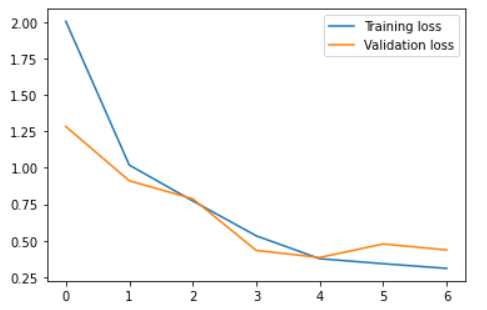
\includegraphics[scale=0.75]{./images/albertoloss}
	\caption{Training-Validation Loss}
  \end{minipage}
  \hfill
  \begin{minipage}[b]{0.45\textwidth}
    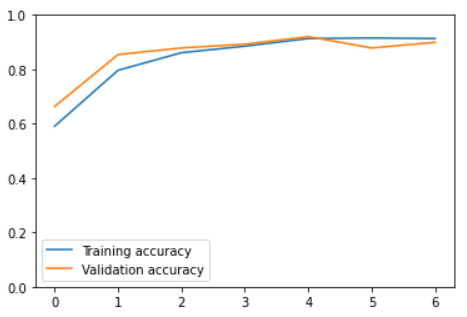
\includegraphics[scale=0.75]{./images/albertoacc}
	\caption{Training-Validation accuracy}
  \end{minipage}
\end{figure}


Los resultados son un poco peores que el modelo de David pero están bastante bien para tratarse de un modelo más simple.\\

Después de haber probado estos modelos podemos llegar a la conclusión de que no es necesario utilizar forzosamente un modelo preentrenado para afrontar este problema, ya que conseguimos unos resultados interesantes desde un enfoque más simple. No obstante, para obtener el mejor modelo posible sí que es recomendable usar modelos preentrenados, como hemos visto con DenseNet o Xception.

\section{Análisis del modelo: mapas de activación, mapas de calor y conclusiones}

Un aspecto que hace que las redes neuronales sean utilizadas con mucha discreción en cualquier ámbito del conocimiento es porque son vistas como cajas negras las cuales no se sabe muy bien qué aprenden y sobre qué características concretas basan sus decisiones, con lo que es necesario que haya algún otro criterio que sea capaz de apoyar la decisión que aporta una red neuronal. Esto pasa con todas las redes, y por tanto también ocurre con las redes neuronales convolucionales. \\

Nuestro objetivo en esta sección es intentar comprender un poco mejor qué características aprenden nuestras redes y qué elementos de la imagen consideran más importantes a la hora de tomar su decisión.  La motivación que tenemos para hacerlo es debido a que en nuestras imágenes tenemos otros elementos que no pertenecen al aparato respiratorio, y que podrían estar afectando negativamente a las decisiones que toman nuestras redes. Puesto que además usamos redes preentrenadas, puede que parte de las características que se detecten debido a dicho preentrenamiento sean reconocidas en lugares de la imagen que no sean del aparato respiratorio. Podrían ser elementos óseos o, de forma más problemática, letras que aparecen en algunas de las imágenes de nuestro conjunto de datos, las cuales son añadidas por algún programa tras haber obtenido la imagen radiográfica inicial.  Si la decisión que toma nuestra red estuviera basada en gran medida en dichas características, independientemente de los buenos resultados que diera esa red, sería indeseable y deberíamos descartarlos, puesto que estaría sobreajustando al conjunto de datos usado directamente, y encima usando características nada relevantes para la tarea que nos compete.


\subsection{Mapas de activación}

Pensamos que una muy buena forma de visualizar cómo ha aprendido la red es viendo los mapas de activación de algunas de sus capas frente a una entrada. De esta manera podremos ver qué filtro sufren mayor activacion, cuáles menos, y en qué zonas. De esta manera se podría llegar a intuir determinadas zonas de la imagen que son relevantes a la hora de hacer una determinada predicción.  Además se podrá ver también de qué forma se va manipulando y transformando la entrada conforme va pasando a lo largo de la red, desde el comienzo que será la imagen original hasta las últimas capas donde la información queda resumida en imágenes muy pequeñas donde el valor de cada pixel condensa una alta información y donde ya no se llega a distinguir la forma original de la imagen.\\

Puesto que hay muchas capas en la red Xception, y además hay bastantes canales por capa, hemos decidido restringir la salida de los mapas de activación a sólo unas determinadas capas, algunas de la parte superior de la red, otras de la parte media de la red y otras de la parte final de la red,  para intentar vislumbrar los hechos que acabamos de decir.\\

Seleccionando 4 capas distribuidas a lo largo de la red hemos obtenido los siguientes resultados (las capas están ordenadas de menor a mayor profuncidad):\\

\begin{figure}[H]
  \centering
    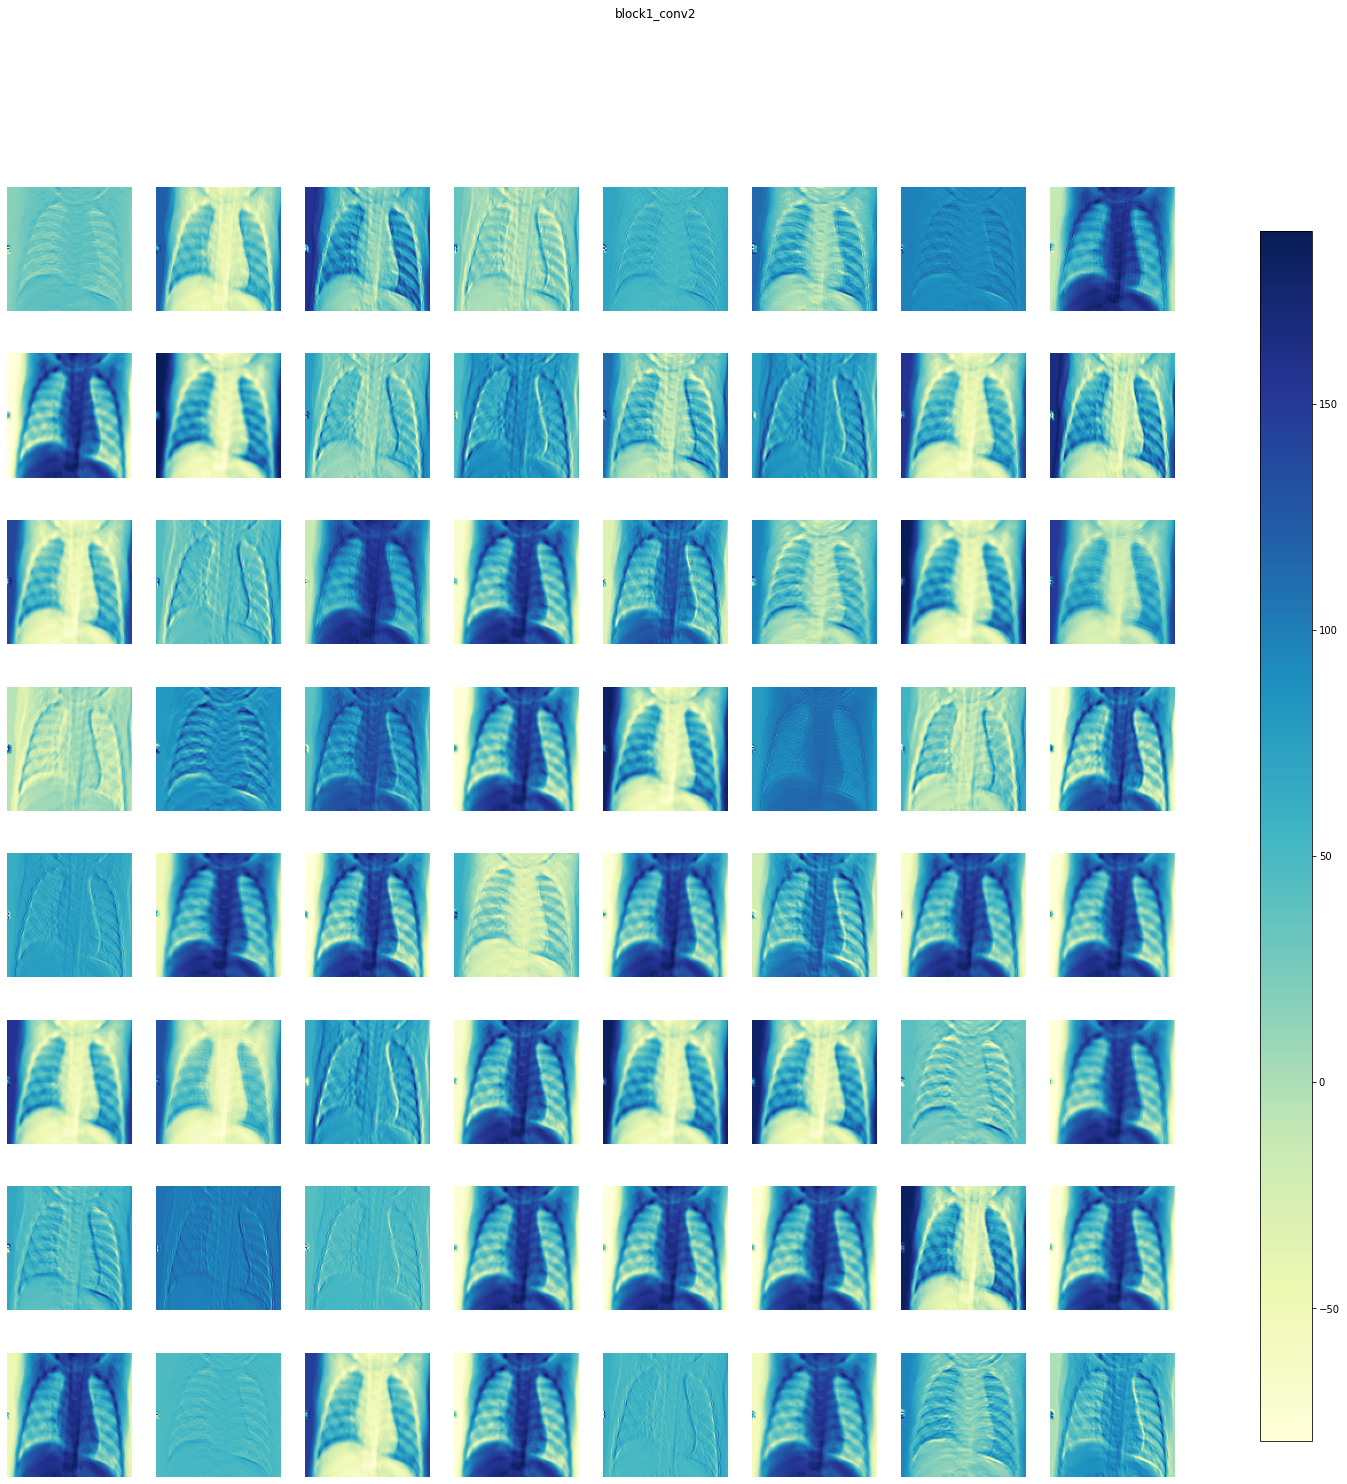
\includegraphics[scale=0.3]{./images/actmap}
	\caption{Mapa de activación para la capa block1\_conv2}

\end{figure}

\begin{figure}[H]
  \centering
    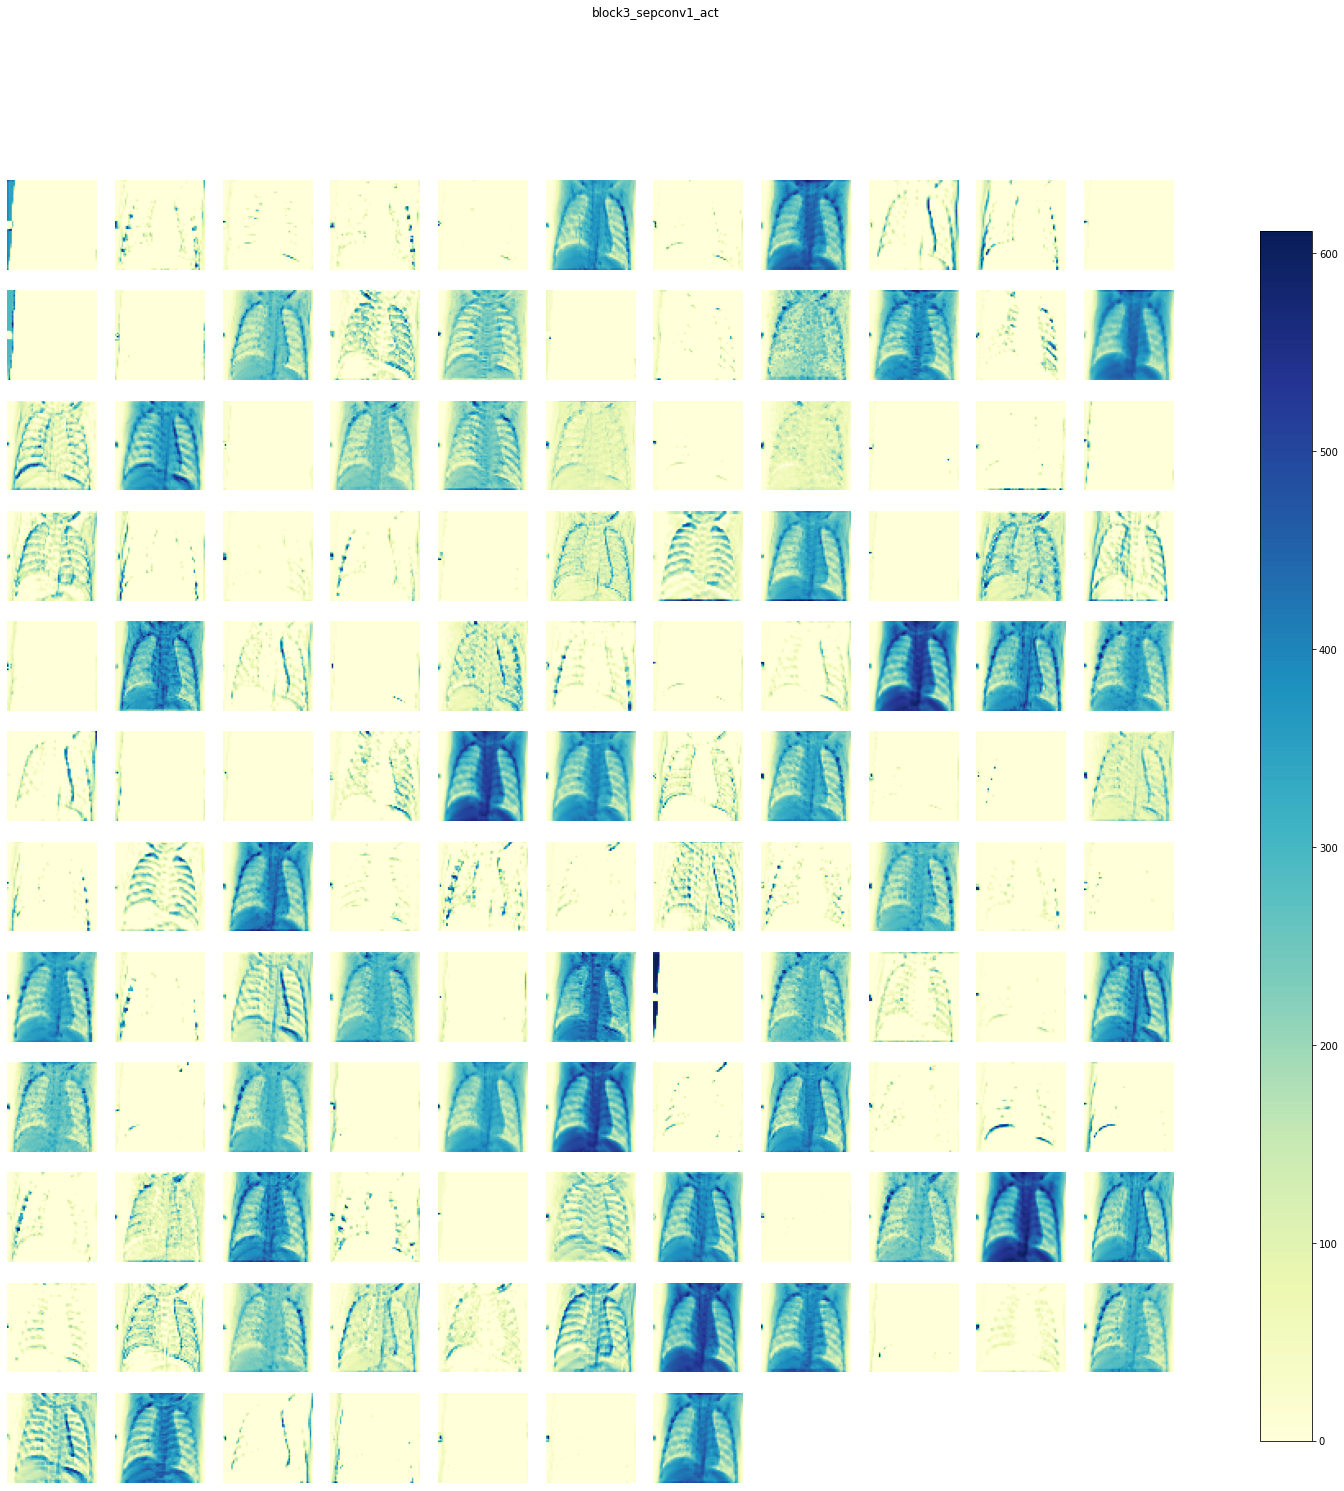
\includegraphics[scale=0.3]{./images/actmap2}
	\caption{Mapa de activación para la capa block3\_sepconv1\_act}

\end{figure}

\begin{figure}[H]
  \centering
    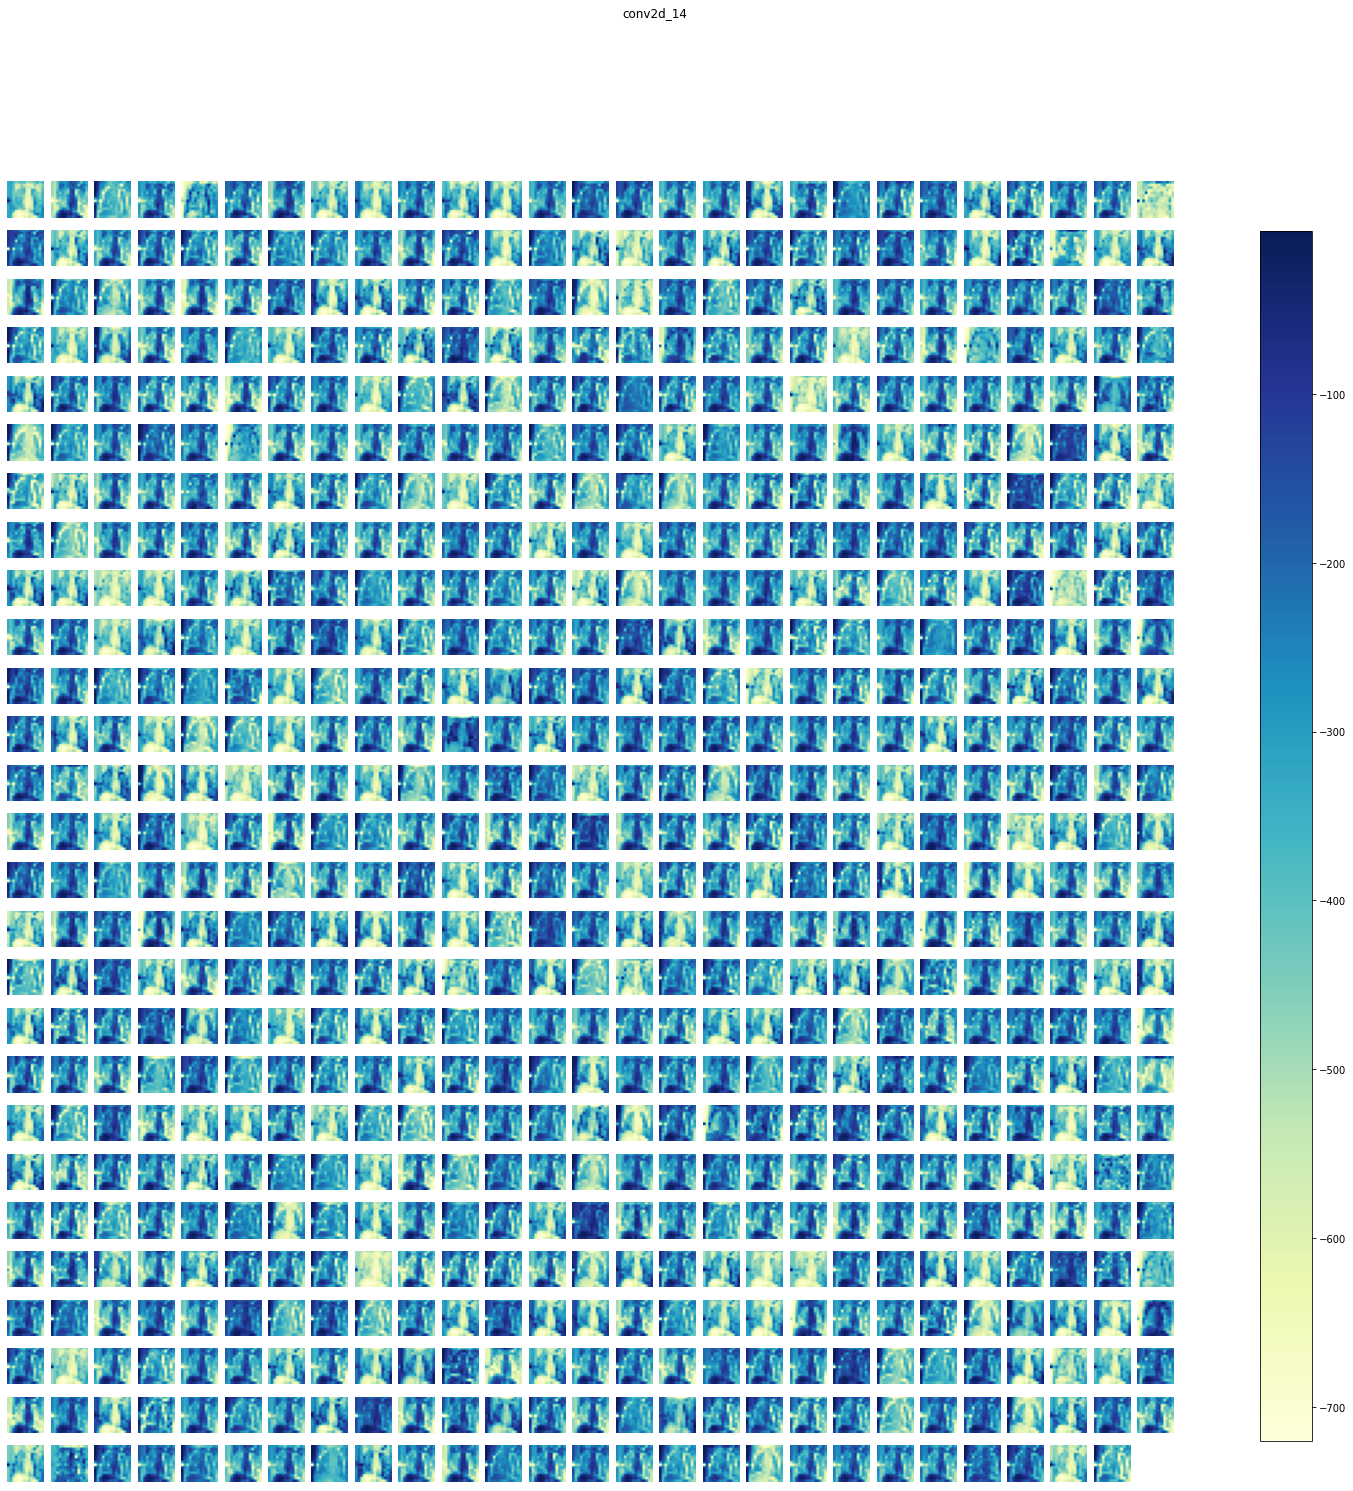
\includegraphics[scale=0.3]{./images/actmap3}
	\caption{Mapa de activación para la capa conv2d\_14}

\end{figure}

\begin{figure}[H]
  \centering
    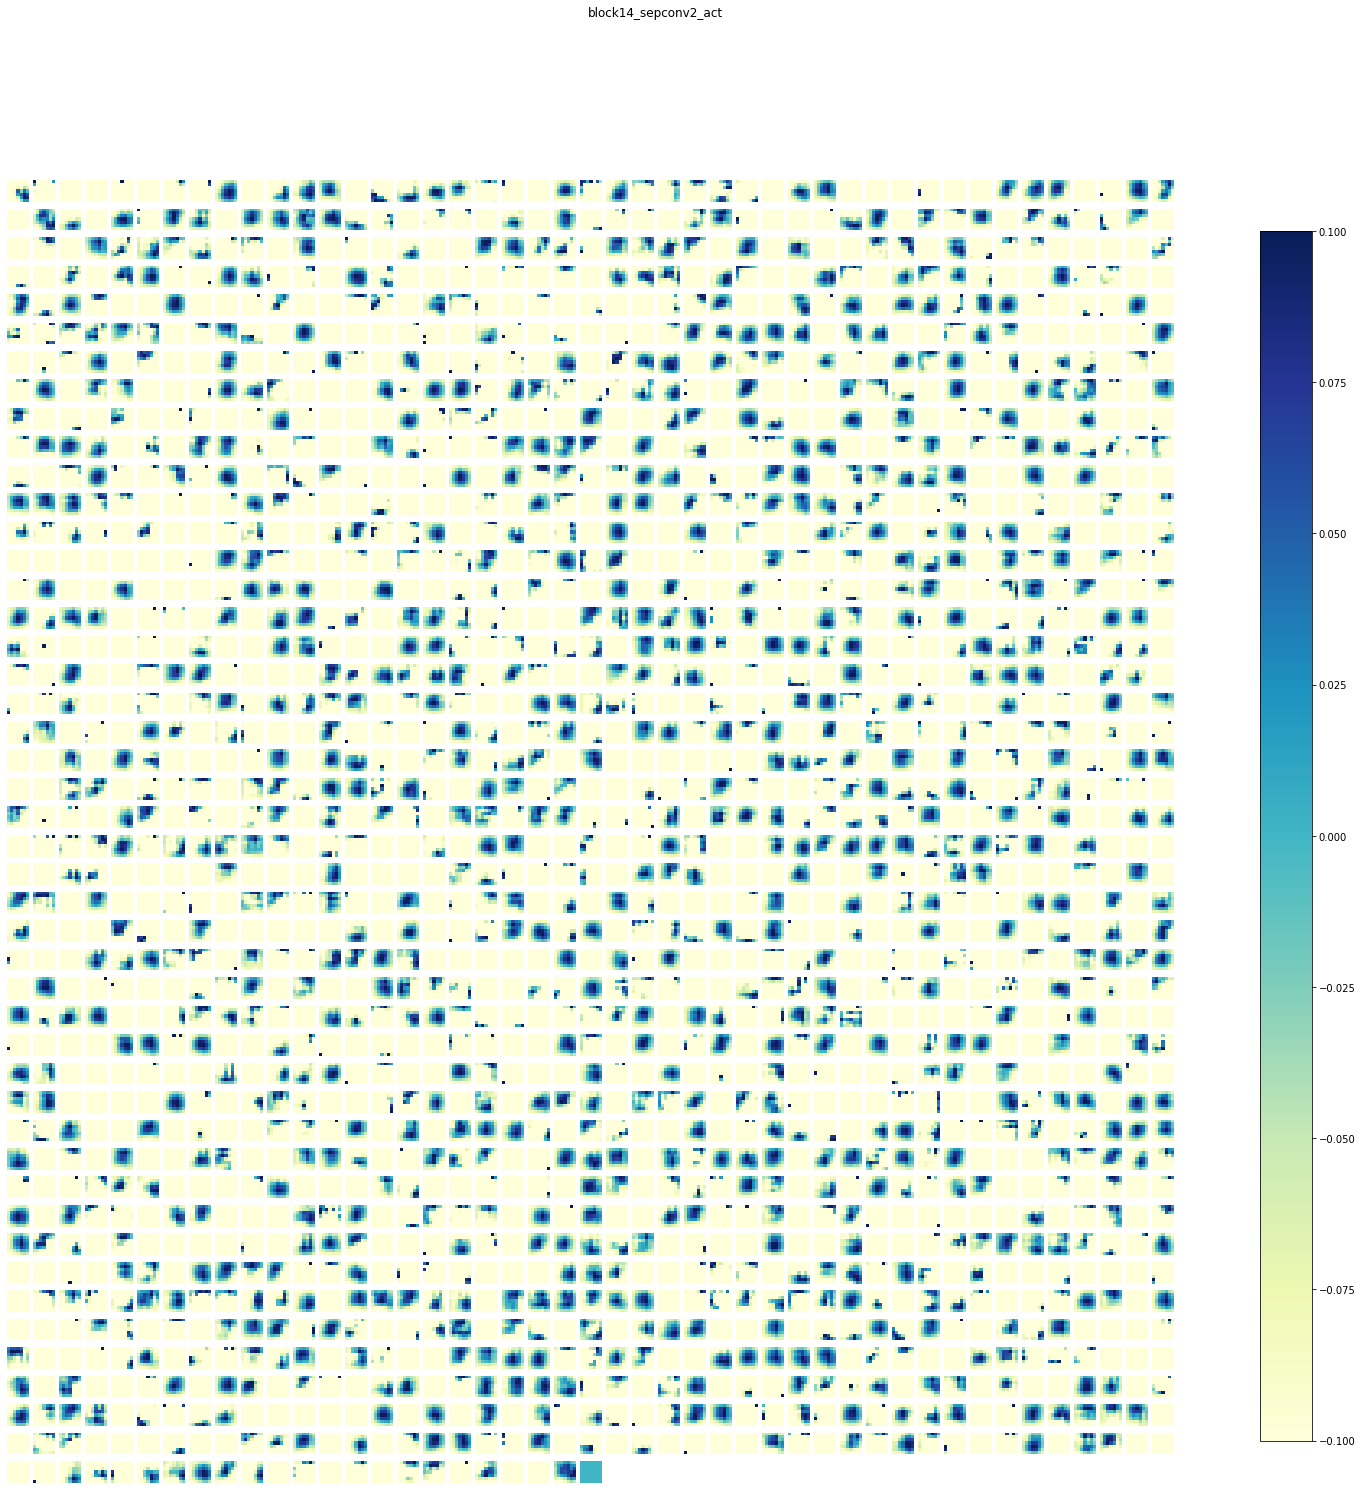
\includegraphics[scale=0.3]{./images/actmap4}
	\caption{Mapa de activación para la capa block14\_sepconv2\_act}

\end{figure}


Como podemos comprobar: INCLUIR RESULTADOS AQUÍ

\subsection{Mapas de calor}


Un mapa de calor es una representación a nivel de imagen de qué zonas de la imagen inicial han sido más relevantes e influyentes a la hora de tomar la decisión por parte de la red neuronal. Dicho de otra forma, el mapa de calor expresa ``en qué zonas de la imagen se ha fijado la red" para tomar su decisión. De esta manera podremos comprobar que la red focaliza su atención en el aparato respiratorio, y además, en qué zonas del mismo lo hace, para intentar esclarecer un poco qué partes del mismo son las más discriminantes a la hora de hacer la tarea de clasificación que nos concierne.  También pudiera ser como hemos dicho antes que la red fijara su atención en algunas imágenes en zonas indeseables, en cuyo caso la red debería ser descartada puesto que automáticamente sobreentrena respecto a los ejemplos de la base de datos, y tendría una capacidad muy baja de generalización y con una gran fuente de errores por hechos externos.\\

Para la implementación del mapa de calor, hemos utilizado el método GRAD-CAM.  En lo que se basa este método es en computar los gradientes respecto a los valores que se han predicho en la última capa convolucional del modelo. Una vez que lo calculamos, lo que hacemos es un resize al tamaño de la imagen original, y superponemos la imagen original con el heatmap para que se vea claramente la zona donde se activa.  Pondremos mapas de colores distintos para el heatmap sobre la última capa convolucional (estilo viridis),  y para la superposición con la imagen original (estilo jet).\\

Vamos a ver el mapa de calor para dos de los modelos anteriores. En concreto para ResNet50 en su versión con los pesos fijos (ResNet-EC) y para el mejor que hemos obtenido, Xception con fine tunning (Xception-FT). Ambos sono modelos con un alto nivel de accuracy, y aunque con Xception-FT se han conseguido los mejores resultados,  el 88\% de accuracy que se conseguía con ResNet-EC no está mal viéndolo en términos absolutos, aunque es muy mejorable en términos relativos.  Queremos compararlos a ver si la diferencia entre sus resultados se basa en que focalizan su atención en distintas partes de la imagen de entrada, o si por el contrario se fijan en las mismas partes de la imagen y fuera por otro motivo.

\subsubsection{Mapas de calor para ResNet-EC}

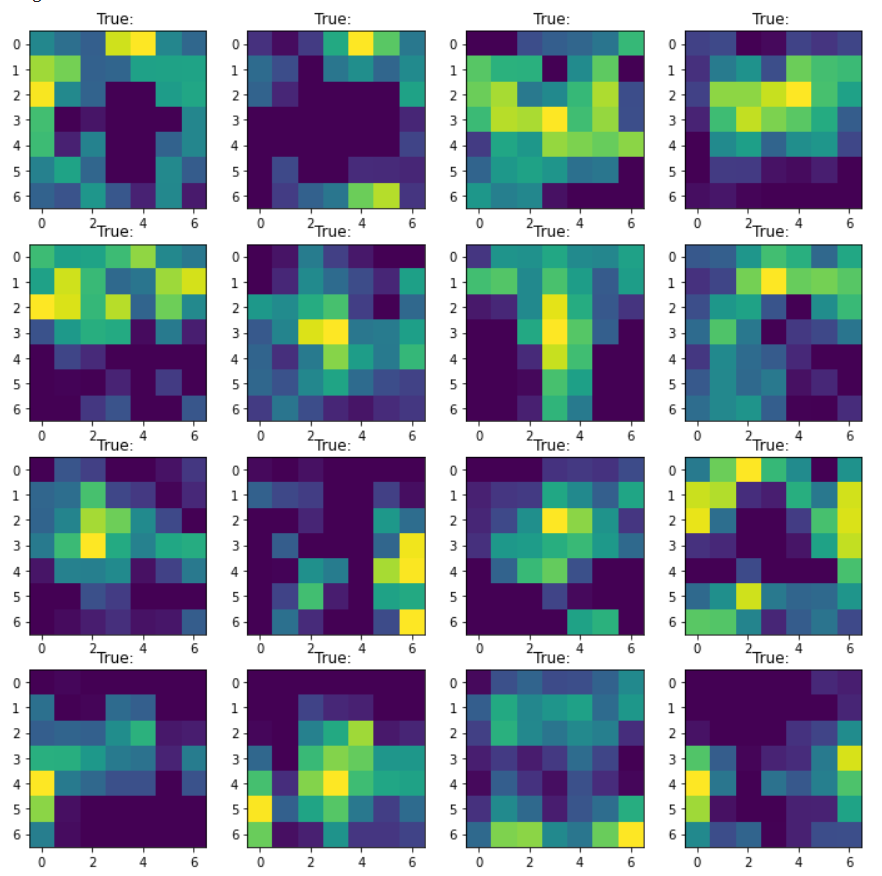
\includegraphics[width=0.85\textwidth]{./images/resnetfilters}

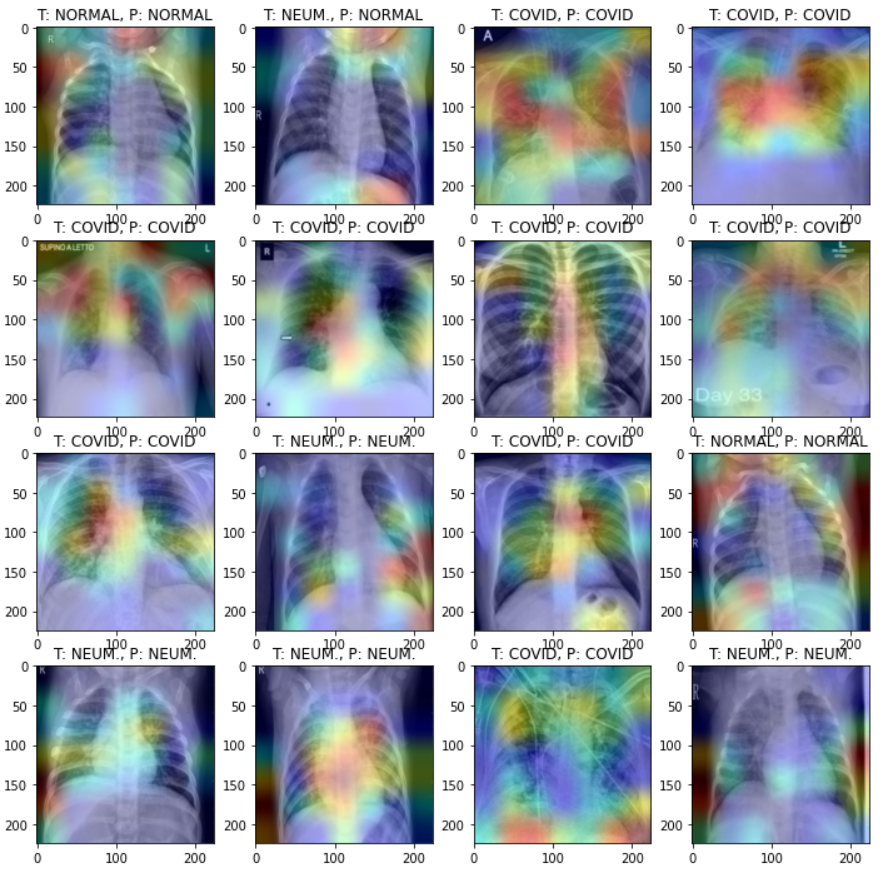
\includegraphics[width=0.85\textwidth]{./images/resnetheatmap}

\subsubsection{Mapas de calor para Xception-FT}

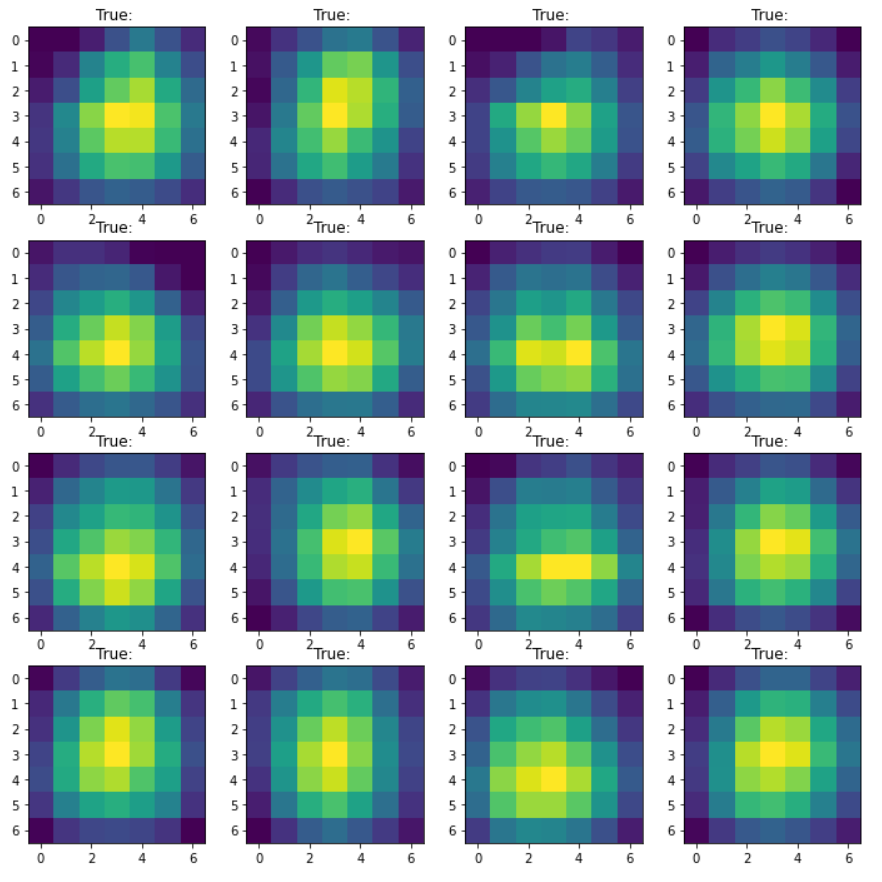
\includegraphics[width=0.85\textwidth]{./images/xceptionfilters}

\includegraphics[width=0.85\textwidth]{./images/heatmapxception}



\subsubsection{Conclusiones}

Si comparamos las dos salidas obtenidas, podemos apreciar claramente una diferencia notable.  Achacamos el hecho de que en el primer modelo la red se fije en numerosas ocasiones en lugares donde no debería fijarse, tales como las letras o diferentes zonas óseas como ya temíamos debido a lo que hemos comentado de que las características que la red tiene aprendidas se detectan en dichas zonas y estropea el proceso de extracción de características.\\

En cambio, para el segundo modelo podemos apreciar que la red se centra en la zona central de las imágenes, que es justo el lugar de ella donde aparece la información más valiosa, evitando los bordes y esquinas donde la información es la misma en todas las clases.  Por lo tanto, aumenta nuestra confianza en el modelo de que sea capaz de adaptarse a otro tipo de datos externos, puesto que se fija en la zona que de antemano sabemos que es donde se puede determinar la clase de una imagen.  Por tanto no es sólo un mejor modelo en cuanto a precisión, sino que también entendemos que tiene mayor criterio a la hora de hacerla. Además, con esto podemos comprobar cómo se centra en la zona pulmonar,  en una zona media-baja de los pulmones.  No sube hasta la zona de la tráquea en casi ninguna ocasión. Así podemos delimitar la zona más discriminante de las imágenes del modelo.

\section{Posibles propuestas de mejora}

Como posibles propuestas para mejoras del modelo se podrían tratar los siguientes aspectos:

\begin{itemize}
\item Modificar diferentes conjuntos de hiperparámetros de la redes , como por ejemplo parámetros del data augmentation o dropout y seleccionar el conjunto para el que el conjunto de hiperparámetros que en validación haya dado mejores resultados.  Puesto que hemos probado muchas redes, el tiempo de ejecución hubiera crecido bastante, pero reconocemos que todavía hay margen de mejora empleando el conjunto de validación para poder optimizar más los resultados de la red variando los hiperparámetros. Actualmente aunque dividimos los datos de entrenamiento sacando un subconjunto para validación, realmente no explotamos el potencial que tiene el conjunto de validación.
\item Se podría haber hecho una comparación más exhaustiva entre los distintos modelos con el objetivo de seleccionar el mejor con mayor garantías utilizando por ejemplo K-fold CV como protocolo experimental. Además, para obtener el mejor modelo posible para cada caso, podríamos haber usado early stopping en lugar de fijar un número concreto de épocas.
\item Se podrían incluir más técnicas de visualización, como por ejemplo calcular las top n patches para algunas de las neuronas de la red, con el objetivo de ver qué regiones de las imágenes han dado mayor valor de activación para esas neuronas. Seleccionando algunas neuronas situadas cerca de la capa de clasificación, cuyo campo receptivo sería prácticamente toda la red, podremos observar cuáles son las imágenes que más claramente dan signos de ser normales, tener covid, o tener otro tipo de neumonías víricas, cosa que sería muy interesante para establecer los ejemplos más característicos de cada conjunto. Además podríamos seleccionar neuronas más alejadas de las capas finales, que tengan un campo receptivo menor, para ver qué patrones de medio tamaño se reconocen en la red que luego serán útiles para la clasificación, ya que facilitaría mucho también el encontrar patrones en una imagen que fueran determinante a la hora de decidir la clase de una imagen.
\item Como hemos podido observar en los mapas de calor, cuando usamos una red preentrenada como extractor de características,  las redes neuronales focalizan su atención en muchas ocasiones en distintas zonas de la imagen que muy poco o nada tienen que ver con los pulmones, donde es evidente que es donde se puede deducir la presencia o no de enfermedad,  tal y como lo muestran los modelos de fine tuning que hemos podido visualizar por mapas de calor.  Lo que podríamos hacer es forzar a nuestro modelo a prestar atención a los pulmones en vez de a los bordes de la imagen, los cuales normalmente tienen letras u otros elementos perniciosos. Para ello podríamos intentar oscurecer los bordes de la imagen,  redimensionar la agrandándola y recortarla dejando fuera los bordes, o podríamos utilizar algún método más sofisticado donde pudiéramos reconocer y eliminar las letras, para posteriormente hacer una reconstrucción de la imagen.  Existen muchas alternativas para forzar a que la red preste atención a la zona pulmonar. Esto no va en contra de la filosofía de las redes neuronales, en cuanto a que ellas deciden qué patrones aprender a reconocer reconocer, puesto que lo único que hacemos es focalizar su atención en la zona de la imagen que nosotros queremos.
\end{itemize}

\cleardoublepage

\phantomsection

\addcontentsline{toc}{section}{Referencias}
\bibliography{bibliograph}
\bibliographystyle{unsrt}




\end{document}
